%%%%% NXT_tutorial %%%%%
%%%%%%%%%% PREAMBLE %%%%%%%%%%
\documentclass[12pt]{article}
\usepackage{amsmath}
\usepackage{graphicx}
\usepackage{wrapfig}
\usepackage{verbatim}
\usepackage[top=2.5cm, bottom=2.5cm, left=2.5cm, right=2.5cm]{geometry}
\usepackage[pdftex]{hyperref}
\usepackage{program_article}
%%%%%%%%%% END of PREAMBLE %%%%%%%%%%
\begin{document}
\baselineskip=12pt
\vspace*{-1.5cm}\textbf{}


\centerline{\bf\Large Chapter 9: Control Lego Mindstorms NXT Robots}
\addtocounter{section}{8}

\section{Ch Mindstorms NXT Control Package}
Ch Mindstorms NXT Control Package brings the inherent functionality of the Ch programming language
 to the intelligence and versatility found in the LEGO Mindstorms NXT robotic design system.
\\
\newline
The Ch Mindstorms NXT Control Package consists of a set of API functions enabling programmers to 
write programs in C or C++ that can access and control the many features of the LEGO Mindstorms 
NXT controller. The API converts the complex messaging tasks required to communicate with the NXT 
into easy to use functions; allowing the user  to focus their efforts on their robotic application, 
rather than the details of communication. The API of the Ch Mindstorms NXT Control Package was designed 
to support and augment all of the functionality found in the LEGO Mindstorms NXT controller. The Ch package 
further enhances the capabilities of the NXT controller by adding data collection and plotting capabilities. 
Additionally an NXT control program, written in C source code can be directly run from any platform in Ch 
without tedious compile/link/execute/debug cycles.
\\
\newline
The communication between the user, the computer, the NXT controller, the sensors, and the motors can be 
described in Figure \ref{fig_NXT_comm}. Once NXT is connected to the computer and a NXT program has started, 
the program instructions are sent from the computer to the NXT. The NXT controller will process these 
instructions perform appropriate tasks by sending commands to the motors or receiving data from the sensors. 
The NXT can collect sensor data and motor encoder counts, and the data can be sent back to the computer for 
further manipulation, display, or stored in the computer for the user. 
\newline
\\
%%%%% START OF FIGURE %%%%%
\begin{figure}[h]
  \begin{center}
    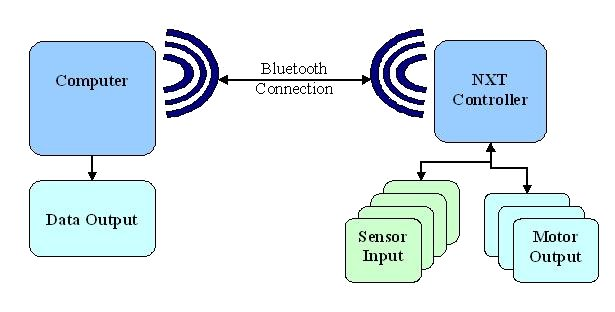
\includegraphics[height=3in]{figure/mindstorm/NXT_connect.png}
    \caption{Communication Diagram of NXT\label{fig_NXT_comm}}
  \end{center}
\end{figure}
%%%%% END OF FIGURE %%%%%
\\
With Ch Mindstorms NXT Control Package, you can quickly develop an NXT robotic application and log your 
results. The ease of design and added functionality makes the Ch NXT Control Package a good candidate for 
any NXT programming application.
\newline
\\
In this chapter, we will go over the basics of a Ch Mindstorms NXT program. We will also discuss about 
how to control a NXT vehicle's motion. Lastly we will describe two demonstration program for the NXT vehicle. 
After reading this chapter, you will be ready to write your own Ch NXT program to control your NXT robot.

%%%%%%%%%%% Basics of a Ch Mindstorms NXT program %%%%%%%%%%
\subsection{Basics of a Ch Mindstorms NXT program}

To successfully control the Mindstorm NXT using Ch, it is important to practice good 
coding habits. The format of the Ch Mindstorm code is very similar to how a normal C
code would be written, with the inclusion of some Ch specific functions and header files 
that are used to connect and control the NXT. The basic structure of a Ch NXT robot 
program is shown in the flow diagram in Figure
    \ref{fig_NXT_pstruc} below.

%%%%% START OF FIGURE %%%%%
\begin{figure}[h!]
  \begin{center}
    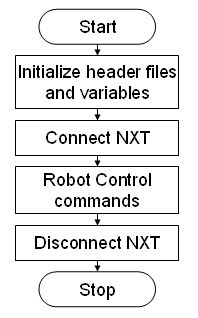
\includegraphics[height=3in]{figure/mindstorm/NXT_pstruc.png}
    \caption{Flow Diagram of a basic NXT program\label{fig_NXT_pstruc}}
  \end{center}
\end{figure}
%%%%% END OF FIGURE %%%%%

\newpage
\subsection{Controlling a NXT Vehicle}
%%%%% START OF FIGURE %%%%%
\begin{figure}[h!]
  \begin{center}
    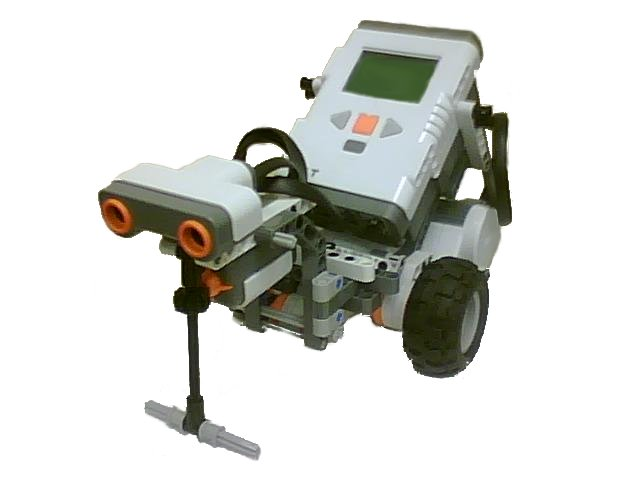
\includegraphics[height=3in]{figure/mindstorm/NXT_vehicle.png}
    \caption{NXT Vehicle\label{fig_NXT_vehicle}}
  \end{center}
\end{figure}
%%%%% END OF FIGURE %%%%%
\noindent
The NXT comes with three actuator output ports and the actuators available are the NXT motors. 
Normaly, you can only control the speed and direction of the connected motors. For a two wheeled NXT vehicle, 
there are two ways that the NXT vehicle can be controlled.  In addition to moving the NXT by controlling the 
individual motors as shown in Figure \ref{fig_NXT_vehicle}, you can also use a set of Ch mindstorm functions
writen specificly to control an NXT vehicle. The diagram of the vehicle and the motor ports 
is shown in Figure \ref{fig_NXT_vehport}. When controlling the individual motors, you would need to define
the speed and direction of each motor.  The functions in the following examples require only a speed. 
In this section, we will show a basic Ch NXT program to move the robot forward. Please make sure your NXT 
vehicle are configured according to to Figure \ref{fig_NXT_vehport} to run our demonstration programs.
\newline
\\
%%%%% START OF FIGURE %%%%%
\begin{figure}[h]
  \begin{center}
    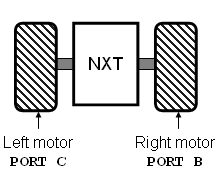
\includegraphics[height=2in]{figure/mindstorm/Vehicle.png}
    \caption{Motor configuration of the NXT Vehicle \label{fig_NXT_vehport}}
  \end{center}
\end{figure}
%%%%% END OF FIGURE %%%%%


\subsubsection{Initialization}
In the beginning of a Ch Mindstorms NXT program or any C program, you must include proper header 
files to run the program properly. Without proper header files, the program will not have the specific 
libraries or source codes to run the program. Essential header files for the NXT includes:
\newline
\\
\begin{verbatim}
    #include <conio.h>
    #include <ch_nxt.h>
    #include <unistd.h>
\end{verbatim}
\noindent
The \verb+conio.h+ is an important header file that include the bluetooth connection functions 
that is required to establish connection between your PC and your NXT. This header also include 
the \_kbhit() function, which is used to detect for hit "anykey" on keyboard if you want to pause 
your program. The \verb+ch_nxt.h+ is the essential header file for Ch NXT function and variables.  
The \verb+unistd.h+ header is needed when using the \verb+sleep()+ function, which is used when 
delays must be placed into a program.
\newline
\\
\subsubsection{Connect the NXT and Checking Connection Status}
The NXT status, sensor/encoder data, and input/output protocols are stored in a structure called \verb+nxt_remote+. 
This structure must be created in every NXT program in order to connect. Therefore, in beginning of your code, 
you must define a \verb+nxt_remote+ structure and use the \verb+nxt_connect()+ function to connect to the NXT. 
The \verb+nxt_connect()+ function will return a 0 if no connection is established, so you will have to terminate 
your program if no connection is established. An example of how to create the \verb+struct+ and how to retrieve 
data are shown below:
\begin{verbatim}
    struct nxt_remote nxtr;

    //Check status of NXT connection
    if (!nxt_connect(&nxtr)){
        printf("Error: Cannot connect to Lego Mindstorm NXT.\n");
        exit(0);
    }

\end{verbatim}
The line \verb+struct nxt_remote nxtr;+ creates the variable \verb+nxtr+ that is used to store data and control the 
NXT robot. The function \verb+nxt_connect()+ called in the if statement is used to terminate the program in 
the event no connection is established. The \verb+printf()+ is included to print out an error message if 
\verb+nxt_connect+ fails. To end the program if connection fails, the function \verb+exit()+ 
is used. The use of \verb+exit(0)+ is similar to the C function \verb+return(0)+, that can be used when no 
\verb+main()+ function is present.
\newline
\\
\subsubsection{Moving the Robot Forward}
After creating a connection with the NXT, you can begin your program to control the NXT. You can move the NXT vehicle 
forward by using the \verb+nxt_forward()+ and selecting a speed. However the speed of the motors are limited, 
and can only be set from 1 to 100. After using the \verb+nxt_forward()+ function, you might want to allow some time 
for the motor to run by pausing the program for a few seconds. To stop the program from running for a few seconds, 
you can use the \verb+sleep()+ function (each unit is 1 second, i.e. \verb+sleep(1)+ = 1 second pause). 
Figure \ref{fig_NXT_forward} shows the NXT vehicle moving forward by actuating both wheels forward with the same speed, 
which is how the function \verb+nxt_forward()+ works.

%%%%% START OF FIGURE %%%%%
\begin{figure}[h]
  \begin{center}
    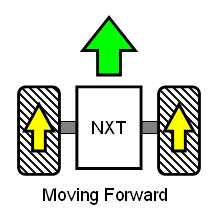
\includegraphics[height=2in]{figure/mindstorm/Vehicle_forward.png}
    \caption{Top-down view of NXT vehicle with two wheels\label{fig_NXT_forward}}
  \end{center}
\end{figure}
%%%%% END OF FIGURE %%%%%

The following shows how the lego vehicle robot is moved forward in the \verb+forward.ch+ program:

\begin{verbatim}
    //Define variables
    int speed = 25;
    //Commands:
    //Move foward
    nxt_forward(speed);
    //Pause program for a while
    sleep(5);
\end{verbatim}

\subsubsection{Ending your program}
After you finish your program, you must end your program properly by stopping all the motors and disconnect 
the NXT from your computer. You can stop the motors using the \verb+nxt_stop()+ function, which stops all of the 
NXT motors. To disconnect the nxt, use the \verb+nxt_disconnect()+ function. For example:
\newline
\\
\begin{verbatim}
    //Stop the motors
    nxt_stop();
    
    //Disconnect NXT
    nxt_disconnect();
\end{verbatim}

\newpage
\subsubsection{forward.ch}
Now that the components of the program have been covered, \verb+forward.ch+ can now be run. The code can 
be written using C or Ch syntax. For simplicity, the following code is presented as a Ch program.

%%%%%%%%%%  program 1 %%%%%%%%%%%%%
%%%%%%%%%%  program of forward.ch %%%%%%%%%%%%%
\verbatiminput{program/demo/forward.ch}
\begin{center}
Program 1: Ch program to move the NXT vehicle forward.
\end{center}
%%%%%%%%%%%%%%%%%%%%%%%%% end %%%%%%%%%%%%%%%%%%%

\subsubsection{How to make your NXT move backward}
For a two wheeled NXT vehicle, you can make the vehicle move backward by using \verb+nxt_backward()+. The function works 
like \verb+nxt_forward()+, moving the robot backwards by entering a speed between 0 to 100. The function works by actuationg 
both wheels backward at the same speed, as shown in Figure \ref{fig_NXT_backward}.
%%%%% START OF FIGURE %%%%%
\begin{figure}[h]
  \begin{center}
    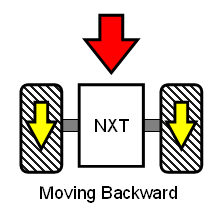
\includegraphics[height=2in]{figure/mindstorm/Vehicle_back.png}
    \caption{NXT vehicle moving backwards\label{fig_NXT_backward}}
  \end{center}
\end{figure}
%%%%% END OF FIGURE %%%%%
Using our new function, we can add the following code fragment to our first program to make the robot move backwards. 
The code fragment is shown below:
\begin{verbatim}
    //Move backward
    nxt_backward(speed);
    sleep(5);
\end{verbatim}
\noindent
The modified program is called: \verb+backward.ch+.
\subsubsection{How to make your NXT move foward and left/right}
To make a two wheeled NXT vehicle to turn left or right while moving, one wheel must be moving 
faster than the other one.  For example, to move the NXT forward and turn left, both wheels will 
have to turn at a positive direction, and the right wheel must run faster than the left wheel. 
Figure \ref{fig_NXT_leftright} shows the NXT vehicle moving forward and left or right by actuating
both wheels forward with different speed.

%%%%% START OF FIGURE %%%%%
\begin{figure}[h]
  \begin{center}
    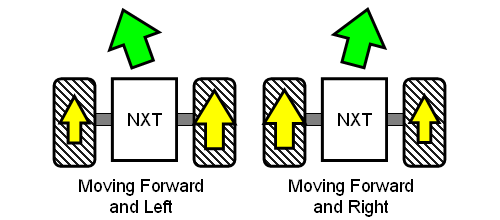
\includegraphics[height=2in]{figure/mindstorm/Vehicle_LR.png}
    \caption{NXT vehicle moving forward and left/right \label{fig_NXT_leftright}}
  \end{center}
\end{figure}
%%%%% END OF FIGURE %%%%%

To make the NXT move forward and left/right, we can use the functions \verb+nxt_turnleft()+ 
and \verb+nxt_turnright()+. Like the previous NXT functions, a speed must be specified when 
using the function.  An example is shown below:
\begin{verbatim}
    //Move Left 
    nxt_turnleft(speed);
    sleep(5);
    
    //or
    
    //Move Right
    nxt_turnright(speed);
    sleep(5);
\end{verbatim}
The modified programs are called: \verb+turnleft.ch+ and \verb+turnright.ch+.
\subsubsection{How to make your NXT turn in place left/right}
To make your NXT vehicle turn or rotate in place, the NXT vehicle wheels must be spun in the opposite direction 
at the same speed. For example, to rotate the NXT vehicle to the left, the right wheel must be spun forward, while 
the left wheel spins at the same speed in reverse. 
Figure \ref{fig_NXT_360LR} shown below shows the NXT vehicle turning in place left or right by actuating the wheels in
    opposite direction.

%%%%% START OF FIGURE %%%%%
\begin{figure}[h]
  \begin{center}
    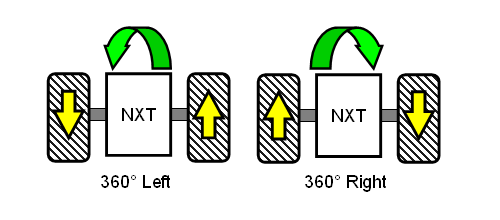
\includegraphics[height=2in]{figure/mindstorm/Vehicle_360LR.png}
    \caption{NXT vehicle turning 360 degrees \label{fig_NXT_360LR}}
  \end{center}
\end{figure}
%%%%% END OF FIGURE %%%%%
\noindent

To make the NXT rotate in place, we can use the functions \verb+nxt_rotateleft()+ 
and \verb+nxt_rotateright()+.  An example of how to use the functions are shown 
below:

\begin{verbatim}
    //rotate left
    nxt_rotateleft(speed);
    sleep(5);
    
    // or
    
    //rotate right
    nxt_rotateright(speed);
    sleep(5);
\end{verbatim}
\noindent
An example program is called: \verb+nxt_turning.ch+.

%%%%%%%%%% NXT Single Motor Control %%%%%%%%%%
\subsection{Advance Mindstorm Motor Control}

The previous section showed simplified controls for an NXT vehicle robot. To control 
alternate NXT designs, or to perform more advance movements with the NXT vehicle, the 
NXT motors must be controlled individually. The following sections shows how to control 
the individual motors, and how the previously presented NXT vehicle actions can be done 
by controlling the individual motors.

\subsection{Motor Control Functions}

The function that is used to control the NXT motors is \verb+nxt_motor()+. To use the function, you need the  
motor port and the motor speed. The speed of the motors are limited, and can 
only ranged from -100 to +100. Like the previous functions, you will need to use the \verb+sleep()+ 
function to leave the motors on for the desired amount of the time. Due to the setup of the NXT 
vehicle, forward motion can be achieved by turning the motors on to the same speed.  For example:

\begin{verbatim}
    //Move foward
    nxt_motor(PORT_B, speed, RUN_IDLE);
    nxt_motor(PORT_C, speed, RUN_IDLE);
    //Pause program for a while
    sleep(5);
\end{verbatim}

This will move the NXT vehicle forward at the value the variable speed was set to. To get the 
NXT vehicle to move in reverse, the same code can be used by changing the sign on speed.
The following shows the \verb+forwardBackward.ch+ rewritten to use the individual motor control.


%%%%%%%%%%  program 2 %%%%%%%%%%%%%
%%%%%%%%%%  program of forwardBackward.ch %%%%%%%%%%%%%
\verbatiminput{program/demo/forwardBackward.ch}
\begin{center}
Program 2: Ch program to move the NXT vehicle forward and backward.
\end{center}
%%%%%%%%%%%%%%%%%%%%%%%%% end %%%%%%%%%%%%%%%%%%%


\subsection{Turning Using Single Motor Control}

Turning and rotation movements can also be achieved using the \verb+nxt_motor()+ functions. As 
previously discussed, to turn our NXT vehicle, one motor must be rotating at a faster speed then 
the other, or the motors must be spinning in the opposite direction. For the following discussion, 
Figures \ref{fig_NXT_leftright} and \ref{fig_NXT_360LR} maybe useful.

To turn the NXT vehicle left, the right wheel must be moving faster in forward direction then the 
left wheel.  The function \verb+nxt_turnleft()+ works by making the left wheel move at 0.7 of the 
speed that the right wheel is set to. To implement it with the single motor control functions, you would  
do the following:

\begin{verbatim}
    //Move foward-left
    nxt_motor(PORT_B, speed, RUN_IDLE);
    nxt_motor(PORT_C, 0.7 * speed, RUN_IDLE);
    //Pause program for a while
    sleep(5);
\end{verbatim}

The value of 0.7 is somewhat arbitrary, and other constant values could be used to test the resulting 
NXT vehicle response. The function \verb+nxt_rotateleft()+ works similarly, instead setting the 
left wheel at the negative speed of the right wheel. An example is shown below:

\begin{verbatim}
    //Rotate left in place
    nxt_motor(PORT_B, speed, RUN_IDLE);
    nxt_motor(PORT_C, -speed, RUN_IDLE);
    //Pause program for a while
    sleep(5);
\end{verbatim}

The \verb+nxt_turnright()+ and \verb+nxt_rotateright()+ work similarly to \verb+nxt_turnleft()+ 
and \verb+nxt_rotateleft()+, with only the commands to the motors reversed. Once you understand 
how the single motor commands work, more advance movements can be done, such as a move back and left 
motion.  The single motor commands can also be used to add a third motor attachment to the NXT 
vehicle, or used to control alternate robot designs that move or act differently.
\newline
\\
One alternative approach to implementing turning is to increase the speed of a wheel, instead of 
decreasing a wheel speed. For example, to implement a left turn, we could increase the speed of 
the right wheel by multiplying by a constant, such as 1.2.  The resulting code would look like:

\begin{verbatim}
    //Move foward-left
    nxt_motor(PORT_B, 1.2 * speed, RUN_IDLE);
    nxt_motor(PORT_C, speed, RUN_IDLE);
    //Pause program for a while
    sleep(5);
\end{verbatim}

While this would work for slower motor speeds, a bug would occur if the NXT vehicle speed was 
set too high. Can you spot why? As previously discussed, the valid motor speeds for the NXT 
motors are between -100 to +100. If the speed variable is set to 100, the command to control 
the left motor (Port C) will function correctly.  The right motor (Port B) will recieve a 
command telling it to set the motor speed to 1.2 x 100 = 120. This is an invalid motor 
command, and if you tried to run it on the NXT, it will cause the motor to reverse direction, 
making the NXT vehicle turn right instead of left. It is important to be watchful of these 
type of errors while writing code to control the NXT.
\newline
\\


%%%%%%%%%% NXT RTC %%%%%%%%%%
\subsubsection{Manual Real Time Control Program}
Manual real time control program allows you to control your NXT vehicle with your keyboard like a 
    remote control.
For a manual control program, a user interface is usually used to display all the possible option
    that a user can input into the program.
The user interface allow the user to know how to control the NXT's motion.
The NXT vehicle RTC program prints out a user interface for the user to use while executing the program.
Figure \ref{fig_NXT_GUI} is the user interface of the NXT vehicle RTC program.
%%%%% START OF FIGURE %%%%%
\begin{figure}[h]
  \begin{center}
    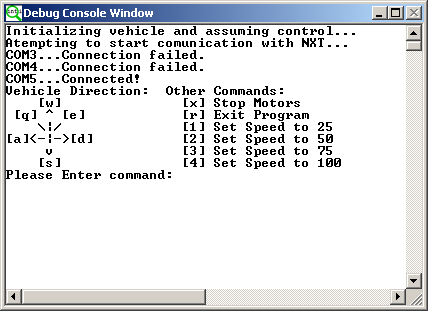
\includegraphics[height=3in]{figure/mindstorm/RTC_GUI.png}
    \caption{NXT vehicle RTC User Interface \label{fig_NXT_GUI}}
  \end{center}
\end{figure}
%%%%% END OF FIGURE %%%%%
\newline
\\
In Figure \ref{fig_NXT_GUI}, the user interface of the NXT vehicle RTC program display all the possible key that the user can use.
In addition, the user interface also indicate the functionality of the key that is being pressed.
When a specific key is pressed during the execution of the NXT vehicle RTC program, the program uses a \verb+switch()+
    statement to performs a fragment of code that send commands to the NXT.
For example:
\begin{itemize}
\item The key \verb+"w"+ is to control the NXT to move forward.
\item The key \verb+"s"+ is to control the NXT to move backward.
\item The key \verb+"a"+ is to control the NXT to turn left.
\item The key \verb+"d"+ is to control the NXT to turn right.
\item The key \verb+"x"+ is to stop the NXT motors.
\item The key \verb+"1"+ is to set the NXT motor speed to 25.
\item The key \verb+"r"+ is to exit the manual RTC program.
\end{itemize}
\noindent
In the robot control code block, a while loop is implemented to allow the user to control the NXT
    continuously until the program is terminated.
Within the while loop, the program grabs the user's input and decide what to do with it using
    the \verb+switch+ and \verb+case+ statements.
The whole NXT vehicle RTC program is shown in Program 2.
Please make sure your NXT vehicle are configured according to to Figure \ref{fig_NXT_vehport} to run Program 2.
In the rest of this section, we are going to explain the whole program in detail.

%%%%% Program 2 %%%%%
\verbatiminput{program/mindstorm/vehicle_rtc.ch}
\begin{center}
Program 2: Manual Real Time Control Program for NXT vehicle.
\end{center}
%%%%% End of Program 2 %%%%%%

\subsubsection*{Header files}
Similar to any C program, you will have to include necessary header files, which is described in the first four
    lines.
    
\begin{verbatim}
    #include <conio.h>
    #include <stdio.h>
    #include <ch_nxt.h>
    #include <unistd.h>
\end{verbatim}

\begin{itemize}
\item The header \verb+conio.h+ provides a function for the program to detect a key press for the
    \verb+-press a key-+ command.
\item The header \verb+stdio.h+ provides input and output function for the program.
    These input and output function allows the program to display output for the user or ask for the user input.
\item The header \verb+ch_nxt.h+ provides the program with general functions of the Ch Mindstorm Control Package.
\end{itemize}

\subsubsection*{Declaring variables}
After including the headers, the C program will start the \verb+main()+ program.
Like any C programs, you must declare variables before you can use them.
On the top few lines of the \verb+main()+ program, variables are declared.
\begin{verbatim}
    struct nxt_remote nxtr;
    int speed = 25,	//speed of the motors. (default to 25)
        quit = 0,	//used by quit case to exit the loop
        status1,	//used to check for errors
        status2;	//used to check for errors
    char key = 'x',	//stores the input from the user
        movemode = 'x';//stores the last movement command
\end{verbatim}

\begin{itemize}
\item The \verb+nxt_remote+ struct stores the connection status, sensor data, and motor counter data of the NXT.
\item The integer variable \verb+speed+ stores the speed of the motor.
\item The integer variable \verb+quit+ is used to check if the user wants to quit the program.
\item The integer variable \verb+status1+ and \verb+status2+ are used to check the sensor connection.
\item The character variable \verb+key+ stores the input from the user.
\item The character variable \verb+movemode+ stores the last command that the user used.
\end{itemize}

\subsubsection*{Checking connection}
After declaring variables, the connection of the NXT needs to be checked.
In the next 7 lines of the program, the program checks for the connection of the NXT to the computer.
If the NXT connection fails, the program will quit.
\begin{verbatim}
    //Connect to NXT
    printf("Initializing vehicle and assuming control...");
    if (!nxt_connect(&nxtr)){
        printf("\nPress any key to exit.\n");
        while (!_kbhit()); //wait for keypress
        exit(0);
    }
\end{verbatim}

\subsubsection*{User interface}
Before the beginning of the real time control, the user must be able to know the function of the key they are pressing.
To do this, the program print out a user interface for the user to read. 
In segment of the Program 4 shown below, the NXT vehicle RTC program used \verb+printf()+ command is used to display the
    user interface for the user to read.
\begin{verbatim}
    //GUI display
    printf("Vehicle Direction:  Other Commands:");
    printf("\n    [w]               [x] Stop Motors");
    printf("\n [q] ^ [e]            [r] Exit Program");
    printf("\n    \\|/               [1] Set Speed to 25");
    printf("\n[a]<-|->[d]           [2] Set Speed to 50");
    printf("\n     v                [3] Set Speed to 75");
    printf("\n    [s]               [4] Set Speed to 100\n");
    printf("Please Enter command:");
\end{verbatim}

\subsubsection*{Real time control}
After completing the initiation of the code, which include adding header files, declaring variables,
    checking connection, and displaying the user interface, the real time control of the NXT
    begins with the robot control code block.
In the robot control code block, a while loop is implemented to allow the user to control the NXT
    continuously until the program is terminated.
Within the while loop, the program grabs an input from the user, and then decide what to
    do with the input using the \verb+switch()+ and \verb+case+ statement.
A basic flow diagram of the control loop for the NXT vehicle RTC program is shown in Figure
    \ref{fig_RTC_controlloop} below.
    
\begin{figure}[h]
  \begin{center}
    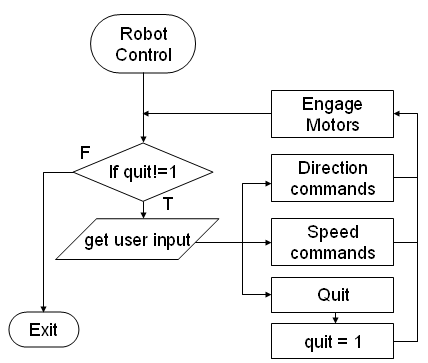
\includegraphics[height=2.4in]{figure/mindstorm/RTC_controlloop.png}
    \caption{NXT vehicle RTC Control Loop Flow Diagram \label{fig_RTC_controlloop}}
  \end{center}
\end{figure}

The program fragment shown below shows the beginning and the end of the while loop for Program 4:
\begin{verbatim}
    while (quit != 1 ) {
        key = _getch();
        switch (key){
        
        ...
        
        }
    }
\end{verbatim}
When the program reaches this stage, the real time control begins. The while loop allows the program 
to keep asking the user's input until the \verb+'r'+ key is pressed. When the \verb+'r'+ key is 
pressed, the program will set \verb+quit+ variable is set to 1, which allows the program to exit 
out of the while loop.\\ \\
\noindent
For first line of the while loop, the program use the \verb+_getch()+ command to obtain a user
 input and store the user input to the variable \verb+key+. After obtaining the user's input in a 
variable, the program use a \verb+switch()+ function to check which key was pressed. Depending on 
what key was pressed, the program will run a fragment of code that sends commands to the NXT.

\subsubsection*{Directional commands}
The movements are controlled using the 'w', 's', 'a', and 'd' format. In Figure \ref{fig_NXT_GUI}, 
the user interface used arrows to indicate the movement direction and associate each direction with 
a specific key. The available buttons for movements are 'w', 's', 'a', 'd', 'q', 'e', and 'x'.
\\ \\
%%% case 'w' %%%
\noindent
When the key 'w' has been pressed, the \verb+switch()+ function will run the codes for the case 'w'.
The program fragment for case 'w' is shown below:
\begin{verbatim} 
    case 'w': //up
        nxt_motor(PORT_B, speed, RUN_IDLE);
        nxt_motor(PORT_C, speed, RUN_IDLE);
        movemode = 'w';
        break;
\end{verbatim}
In case 'w', the program will run the motor in \verb+PORT_B+ and \verb+PORT_C+ forward at the velocity 
\verb+speed+, and then set the motor to run idle mode. Next, 'w' key is stored in the variable 
\verb+movemode+, which will be used to indicate the current mode for NXT vehicle. Basically, the case 
'w' will move the NXT vehicle forward with velocity \verb+speed+.
\\ \\
%%% case 's' %%%
\noindent
When the key 's' has been pressed, the \verb+switch()+ function will run the codes for the case 's'.
The program fragment for case 's' is shown below:
\begin{verbatim} 
    case 's': //down
        nxt_motor(PORT_B, -speed, RUN_IDLE);
        nxt_motor(PORT_C, -speed, RUN_IDLE);
        movemode = 's';
        break;
\end{verbatim}
In case 's', the program will run the motor in \verb+PORT_B+ and \verb+PORT_C+ backward at the velocity 
\verb+speed+, and then set the motor to run idle mode. Next, 's' key is stored in the variable \verb+movemode+, 
which will be used to indicate the current mode for NXT vehicle. Basically, the case 's' will move the NXT 
vehicle backward with velocity \verb+speed+.
\\ \\
%%% case 'a' %%%
\noindent 
When the key 'a' has been pressed, the \verb+switch()+ function will run the codes for the case 'a'.
The program fragment for case 'a' is shown below:
\begin{verbatim} 
    case 'a': //left
        nxt_motor(PORT_B, speed, RUN_IDLE);
        nxt_motor(PORT_C, -speed, RUN_IDLE);
        movemode = 'a';
\end{verbatim}
In case 'a', the program will actuate motor in \verb+PORT_B+ forward at velocity \verb+speed+ and 
actuate motor in     \verb+PORT_C+ backward at velocity \verb+speed+, and then set the motor to 
run idle mode. Next, 'a' key is stored in the variable \verb+movemode+, which will be used to 
indicate the current mode for NXT vehicle.
\\ \\
%%% case 'd' %%%
\noindent
When the key 'd' has been pressed, the \verb+switch()+ function will run the codes for the case 'd'.
The program fragment for case 'd' is shown below:
\begin{verbatim} 
    case 'd': //right
        nxt_motor(PORT_B, -speed, RUN_IDLE);
        nxt_motor(PORT_C, speed, RUN_IDLE);
        movemode = 'd';
        break;
\end{verbatim}
In case 'd', the program will actuate motor in \verb+PORT_B+ backward at velocity \verb+speed+ 
and actuate motor in \verb+PORT_C+ forward at velocity \verb+speed+, and then set the motor to run 
idle mode. Next, 'd' key is stored in the variable \verb+movemode+, which will be used to indicate 
the current mode for NXT vehicle.
\\ \\
%%% case 'q' %%%    
\noindent
When the key 'q' has been pressed, the \verb+switch()+ function will run the codes for the case 'q'.
The program fragment for case 'q' is shown below:
\begin{verbatim} 
    case 'q': //forward-left
        nxt_motor(PORT_B, speed, RUN_IDLE);
        nxt_motor(PORT_C, speed*0.6, RUN_IDLE);
        movemode = 'q';
        break;
\end{verbatim}
In case 'q', the program will actuate motor in \verb+PORT_B+ forward at velocity \verb+speed+ and 
actuate motor in \verb+PORT_C+ forward at velocity 0.6*\verb+speed+, and then set the motor to run 
idle mode. Next, 'q' key is stored in the variable \verb+movemode+, which will be used to indicate 
the current mode for NXT vehicle.
\\ \\
%%% case 'e' %%%
\noindent 
When the key 'e' has been pressed, the \verb+switch()+ function will run the codes for the case 'e'.
The program fragment for case 'e' is shown below:
\begin{verbatim} 
    case 'e': //forward-right
        nxt_motor(PORT_B, speed*0.6, RUN_IDLE);
        nxt_motor(PORT_C, speed, RUN_IDLE);
        movemode = 'e';
        break;
\end{verbatim}
In case 'e', the program will actuate motor in \verb+PORT_B+ forward at velocity 0.6*\verb+speed+ and 
actuate motor in \verb+PORT_C+ forward at velocity \verb+speed+, and then set the motor to run idle 
mode. Next, 'e' key is stored in the variable \verb+movemode+, which will be used to indicate the 
current mode for NXT vehicle.
\\ \\
%%% case 'x' %%%
\noindent
When the key 'x' has been pressed, the \verb+switch()+ function will run the codes for the case 'x'.
The program fragment for case 'x' is shown below:
\begin{verbatim} 
    case 'x': //stop
        nxt_motor(PORT_B, 0, OFF_IDLE);
        nxt_motor(PORT_C, 0, OFF_IDLE);
        movemode = 'x';
        break;
\end{verbatim}
In case 'x', the program will set the motor in \verb+PORT_B+ and \verb+PORT_C+ to zero velocity, and then
    set the motor to off idle mode.
Next, 'x' key is stored in the variable \verb+movemode+, which will be used to indicate the current mode for NXT vehicle.
Basically, the case 'x' stops the motor and keep it turned off until another key is pressed.

\subsubsection*{Speed control}
The speed of the motor is controlled by the number key '1', '2', '3', and '4'.
In Figure \ref{fig_NXT_GUI}, the user interface shows that each key has a specific speed.
For example, key '1' indicates 25 speed, and key '2' indicate 50 speed.
As shown below, each of the key has its fragment of code.

\begin{verbatim}
    case '1': //speed 25
        speed = 25;
        ungetch(movemode);
        break;
    case '2': //speed 50
        speed = 50;
        ungetch(movemode);
        break;
    case '3': //speed 75
        speed = 75;
        ungetch(movemode);
        break;
    case '4': //speed 100
        speed = 100;
        ungetch(movemode);
        break;
\end{verbatim}
\noindent
For each of the case, the fragment of code changes the variable \verb+speed+ and performs an \verb+ungetch()+ command.
The \verb+ungetch()+ command allows the program run the mode that it was previously saved in the variable \verb+movemode+
    before the speed keys are pressed.
Basically, the speed keys allow the program to change the speed of the NXT motor without changing the movement
    mode that it was in.

\subsubsection*{Functions for other keys}
As mentioned before, the while loop allows the program to keep asking the user's input until the variable
    \verb+quit+ is set to 1.
To quit the while loop, we must have a special case that sets the variable \verb+quit+ to 1.
When the key 'r' is pressed, the \verb+switch()+ function will perform a fragment of code for case 'r'.
The program fragment for case 'r' is shown below:
\begin{verbatim}
    case 'r': //quit
        printf("\nExiting program.\n");
        quit = 1;
        break;
\end{verbatim}
\noindent
When the \verb+'r'+ key is pressed, the program will print out the statement 'exiting program' and set \verb+quit+
    variable is set to 1, which allows the program to exit out of the while loop.
\newline
For the keys that is not specified to any cases, a default case is used for the time when the user input a wrong key.
The program fragment for the default case is shown below:
\begin{verbatim}
    default:
        printf("\nInvalid Input!\n");
\end{verbatim}
\noindent
This fragment prints 'Invalid Input!' to the user to indicate the key they just pressed is an invalid input.

\subsubsection*{Disconnecting your NXT}
After the while loop, the NXT vehicle RTC program ends with the four lines shown below.
\begin{verbatim}
    nxt_disconnect();   //stop interfacing. This also stops the motors.
    printf("Press any key to exit.\n");
    while (!_kbhit()); //wait for key press
\end{verbatim}
\noindent
These lines of code stop the NXT motors, disconnect the NXT from the computer, ask for the user
    to press a key, and terminate  the program.
%%%%%%%%%% end of NXT RTC %%%%%%%%%%
%%%%%%%%%%% End of Controlling NXT Vehicle %%%%%%%%%%

%%%%%%%%%%% Using NXT Sensors %%%%%%%%%%
\subsection{Using NXT Sensors}
Sensors converts a physical quantity and convert it to signals which can be read by the NXT or the computer. 
Sensors allows the communication between the outside environment to the NXT. The NXT is equipped with four 
sensor input ports and you can equip each port with a variety of different sensors. In this section, we are 
going to discuss about how to use the touch sensor and the ultrasonic sensor. In these discussion, two 
demonstration program will be presented. Please make sure your NXT vehicle are configured according to to 
Figure \ref{fig_NXT_sensport} to run these demonstration programs.
%%%%% START OF FIGURE %%%%%
\begin{figure}[h]
  \begin{center}
    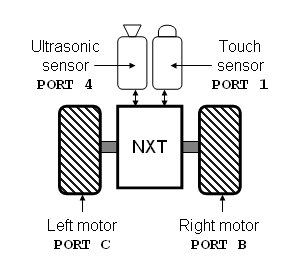
\includegraphics[height=2.4in]{figure/mindstorm/NXT_auto.png}
    \caption{Sensor/Motor configuration of the NXT Vehicle \label{fig_NXT_sensport}}
  \end{center}
\end{figure}
%%%%% END OF FIGURE %%%%%

\subsubsection{Using your touch sensor}
After you have connected your NXT to your PC, you will need to set up the sensor if you would like to include 
sensors in your NXT program. For example, if you want to add components like light sensor, ultrasonic sensor, 
and/or touch sensor, you will need to set up their connection using the \verb+nxt_setsensor()+ function. 
The \verb+nxt_setsensor()+ function will return 0 if no connection is established, so you can terminate the 
program if a sensor connection is not established. An example connection check for adding the Touch and 
Ulstrasonic sensors to the NXT vehicle is as follow:

\begin{verbatim}
    struct nxt_remote nxtr;

    //Check status of NXT connection
    if (!nxt_connect(&nxtr)){
        exit(0);
    }
    
    //Setup sensors and check sensor connection
    int status1=2, status2=2;

    //Save status of PORT_1, and PORT_4
    status1=nxt_setsensor(PORT_1,TOUCH,BOOLEANMODE);
    status2=nxt_setsensor(PORT_4,ULTRASONIC,RAWMODE);
    
    //Check connection status of PORT_1
    if(status1==0) {
        exit(0);
    }
    
    //Check connection status of PORT_4
    if(status2==0) {
        exit(0);
    }
\end{verbatim}
As in previous examples, the nxt\_remote stucture, \verb+nxtr+, is created, and the initial connection 
to the NXT is made. The next step is to initialize the NXT sensor ports to the correct types and ensure 
the sensors are working correctly.  The int variables \verb+status1+ and \verb+status2+ are used to 
check the return value of the function \verb+nxt_setsensor()+.
//
A common application of touch sensors for a vehicle robot is for obstacle detection. In order to 
demonstrate the use of the touch sensor, consider the touch sensor demo in Program 3.

%%%%% Program 3 %%%%%
\verbatiminput{program/mindstorm/touchsensor.ch}
\begin{center}
Program 3: Ch NXT touch sensor demonstration program.
\end{center}
%%%%% End of Program 3 %%%%%%

\subsubsection*{Checking touch sensor connection}
Program 3 is similar to Program 1, the only changes is the addition of the use of the touch sensor. Program 3 
makes the NXT move forward until the touch sensor is triggered, after which it will back up and stop. One of 
the additions that is added in Program 3 is the initialization of the touch sensor. The fragment of the 
initialization of the touch sensor is shown below.

\begin{verbatim}
    //Set sensor types
    int status;
    status = nxt_setsensor(PORT_1, TOUCH, BOOLEANMODE);
    if (status == 0){
        exit(0);
    }
\end{verbatim}
In this fragment, the program use the \verb+nxt_setsensor()+ command to set the touch sensor to \verb+PORT 1+. 
The connection status between the NXT and the sensor is then returned in the variable called status. Next, the 
if statement check if the connection to the sensor is good. If the variable status is equal to 0, which means
 no sensor connection, the program will be exited and the rest of the codes will not be executed.
    
\subsubsection*{Using while loop}
A while loop is a common method that is used for sensor data gathering. For every iteration of the while loop, 
the program checks the data gathered by the touch sensor. After gathering the data, the program decide what to 
do with the data. A simple flow diagram of the while loop of the touch sensor demo program is shown in Figure 
\ref{fig_NXT_touchflow}

%%%%% START OF FIGURE %%%%%
\begin{figure}[h]
  \begin{center}
    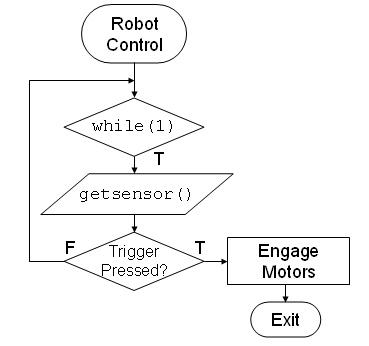
\includegraphics[height=2.4in]{figure/mindstorm/NXT_touchflow.png}
    \caption{Flow Diagram of the while loop in Program 3 \label{fig_NXT_touchflow}}
  \end{center}
\end{figure}
%%%%% END OF FIGURE %%%%%

In Program 3, the while loop checks for the data of the touch sensor. If the touch sensor is triggered, 
the data of the touch sensor will be set to below 500. Then the program will move the NXT backward and 
disconnect the NXT. The while loop of the touch sensor demonstration program is described below:
\begin{verbatim}
    while(1){
        //Get touch sensor data
        nxt_getsensor(PORT_1);
        //If touch sensor is triggered
        if (nxtr.NXT_sensorvalraw[PORT_1] < 500){
            //Move backward
            nxt_motor(PORT_B, -speed, RUN_IDLE);
            nxt_motor(PORT_C, -speed, RUN_IDLE);
            sleep(5);
            break;
        }
    }
\end{verbatim}
In this while loop, the program uses the \verb+nxt_getsensor()+ command to get the data from \verb+PORT 1+, 
which is the port for the touch sensor according to Figure \ref{fig_NXT_sensport}. Next, the program checks 
the touch sensor if it is pressed with the if statement. If the touch sensor has been triggered, the codes 
in the if statement will run. The codes inside the if statement is the same command for moving the NXT 
backward. After moving the NXT backward, the command break allows the program to exit out of the while loop.
 This while loop will never exit until the touch sensor is triggered and the break command is used.

\subsubsection{Using your ultrasonic sensor}
In order to demonstrate the use of the ultrasonic sensor, consider the ultrasonic sensor demo in Program 4.
NOTE: If your robot gets stuck, put your hands in front of the ultrasonic sensor to quit the loop.

%%%%% Program 4 %%%%%
\verbatiminput{program/mindstorm/ultrasonicsensor.ch}
\begin{center}
Program 4: Ch NXT ultrasonic sensor demonstration program.
\end{center}
%%%%% End of Program 4 %%%%%%
\subsubsection*{Checking touch sensor connection}
Like Program 3, Program 4 is meant to be a brief demonstration of one method of using an ultrasonic sensor 
with a vehicle NXT.
Similar to the initialization of the touch sensor, the initialization of the ultrasonic sensor is shown below:

\begin{verbatim}
    //Set sensor types
    int status;
    status = nxt_setsensor(PORT_4, ULTRASONIC, RAWMODE);
    if (status == 0){
        exit(0);
    }
\end{verbatim}
In this program fragment, the \verb+nxt_setsensor()+ command sets the ultrasonic sensor to \verb+PORT 4+.
Next, it checks the return value of the sensor connection status.
The program will quit if the return value is 0, meaning there is no connection between the sensor and the NXT.

\subsubsection*{Contents in the while loop}
In Program 4, the while loop uses the ultrasonic sensor to detect distances between the NXT and the obstacles in 
front of the NXT. The ultrasonic sensor will detect distances and the program code reacts to the data by slowing 
down or speeding up. The flow diagram of the while loop of Program 4 is shown in Figure \ref{fig_NXT_ultraflow}.
%%%%% START OF FIGURE %%%%%
\begin{figure}[h]
  \begin{center}
    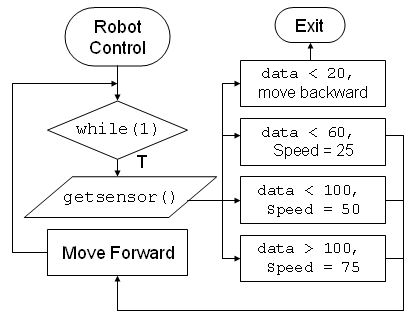
\includegraphics[height=2.4in]{figure/mindstorm/NXT_ultraflow.png}
    \caption{Flow Diagram of the while loop in Program 3 \label{fig_NXT_ultraflow}}
  \end{center}
\end{figure}
%%%%% END OF FIGURE %%%%%

The while loop code block for Program 4 is shown below:
\begin{verbatim}
    //Commands:
    while(1){
        //Get ultrasonic sensor data
        nxt_getsensor(PORT_4);
        //If obstacle is really close
        if (nxtr.NXT_sensorvalraw[PORT_4] < 20){
            speed = 25;
            //Move backward
            nxt_motor(PORT_B, -speed, RUN_IDLE);
            nxt_motor(PORT_C, -speed, RUN_IDLE);
            sleep(3);
            //Quit the while loop
            break;
        }
        //Else if the obstacle is close
        else if(nxtr.NXT_sensorvalraw[PORT_4] < 60){
            speed = 25;
        }
        //Else if the obstacle is not close
        else if(nxtr.NXT_sensorvalraw[PORT_4] < 100){
            speed = 50;
        }
        //Else if there is no obstacle in sight
        else if(nxtr.NXT_sensorvalraw[PORT_4] < 200){
            speed = 75;
        }
        //Sensor value larger than 200
        else{
            speed = 75;
        }
        //Move forward (constantly)
        nxt_motor(PORT_B, speed, RUN_BRAKE);
        nxt_motor(PORT_C, speed, RUN_BRAKE);
    }
\end{verbatim}
\noindent
Similar to Program 3, the while loop in Program 4 also gathers the sensor data using the
    \verb+nxt_getsensor()+ command to gather data from the ultrasonic sensor in \verb+PORT 4+.
Next, the if-else statement block determine what to do depending on the distance data from ultrasonic sensor.
\begin{itemize}
\item If the sensor value is below 20, which means the vehicle is very close to an obstacle, the program tells the
    vehicle to reverse, and then break out of the while loop.
\item If the sensor value is above 20 and below 60, which means the vehicle is close to an obstacle, the
    program set the speed variable to 25.
\item If the sensor value is above 60 and below 100, which means the vehicle is not close to an obstacle, the
    program set the speed variable to 50.
\item If the sensor value is above 100 and below 200, which means there is nothing in front of the vehicle,
    the program set the speed variable to 75.
\item If the sensor value is other value that is not mentioned above, the program set the speed variable to 75.
\end{itemize}
After the if-else statement block, the program sets the robot to move forward with velocity set at the speed variable.
Then the program returns back to the beginning of the while loop, which is to gather data from the sensor again.

%%%%%%%%%% NXT auto %%%%%%%%%%
\subsubsection{Autonomous Control Program}
In the previous sections, we thoroughly covered the manual real time control program, which allows you to 
remote control your NXT vehicle with your keyboard.
In this section, we will talk about the autonomous control program for the NXT vehicle.
In an autonomous control program, the robot, which is the NXT, must be able to move around by itself without
    human commands or interventions.
In order to achieve such task, the NXT must be able to detect obstacles using its sensors and steer away from the
    obstacle using its actuators.
A typical autonomous control scheme is to sense, plan, and act, which is shown in Figure \ref{fig_NXT_SPA}.
%%%%% START OF FIGURE %%%%%
\begin{figure}[h]
  \begin{center}
    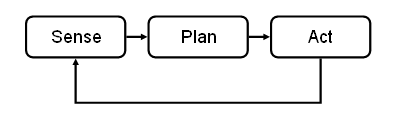
\includegraphics[height=1in]{figure/mindstorm/Senseplanact.png}
    \caption{Sense Plan Act Diagram \label{fig_NXT_SPA}}
  \end{center}
\end{figure}
%%%%% END OF FIGURE %%%%%
\begin{itemize}
\item Sense is to gather data from the robot's surrounding.
\item Plan is to plan the interaction between the robot and its surrounding using gathered data.
\item Act is to act with robot's surrounding.
\end{itemize}
The main difference between the manual RTC program and the autonomous program is the content inside the while loop.
In the manual RTC program, the codes inside the while loop scan for user's input and the robot acts on the input that
    the user provided.
In the autonomous program, the codes inside the while loop perform the sense-plan-act cycle similarly to the diagram
    shown in Figure \ref{fig_NXT_SPA}.
Every cycle, the information is gathered from the sensor and send back to the computer.
The computer will decide what to do depending on the sensor data.
The autonomous control program for the NXT vehicle is described in Program 5.
%%%%% Program 5 %%%%%
\verbatiminput{program/mindstorm/vehicle_auto.ch}
\begin{center}
Program 5: Autonomous Control Program for NXT vehicle.
\end{center}
%%%%% End of Program 5 %%%%%%
In Program 5, the sensors that is used are the touch sensor and the ultra sonic sensor.
These sensors are located in the front of the vehicle so that when the vehicle encounters an obstacle, the program will
    control the robot to avoid or steer away from it.
A diagram of the vehicle and its sensor and actuators of the program is shown in Figure \ref{fig_NXT_sensport}.
Please make sure your NXT vehicle are configured according to to Figure \ref{fig_NXT_sensport} to run Program 5.

\subsubsection*{Exiting the while loop}
In the autonomous program, there must be codes that allow the user to quit the autonomous program.
Otherwise, the robot will roam forever until the batteries run out or until a deliberate shut down of the program.
In the beginning of the while loop, the program checks for the user's input. 
If the user's input is 'q' to quit, then the program will break out of the while loop and safely disconnects the NXT.
If the user's input is not 'q' or if the user did not input anything, the program will continue to the next section of
    the while loop.
The program fragment for exiting the autonomous program is shown below.
\begin{verbatim}
    //check user input 'q' to quit
    if(kbhit()){
        if (getch()=='q'){	
            printf("\nExiting.");
            break;
        }
    }
\end{verbatim}
In this program fragment, an if statement is used to check if a keyboard key has been hit.
Next, if a keyboard key has been hit, another if statement checks if the input is 'q'.
If both conditions are satisfied, the break statement will break out of the while loop of the program.

\subsubsection*{Touch sensor}
The next section of the while loop uses the touch sensor to control the NXT vehicle.
When the NXT contact some obstacle in the front, the touch sensor will be triggered.
The autonomous program will notice that the touch sensor is triggered and command the NXT to steer away from the obstacle.
The program fragment of the touch sensor is shown below.
\begin{verbatim}
    //get touch sensor. If pressed reverse and turn left
    nxt_getsensor(PORT_1);
    if (nxtr.NXT_sensorvalraw[PORT_1]<500){
        nxt_motor_rotate(PORT_B,-25,720);
        nxt_motor_rotate(PORT_C,-25,720);
        sleep(1);
        nxt_motor(PORT_B,0,RUN_BRAKE);
        nxt_motor(PORT_C,0,RUN_BRAKE);
        sleep(.750);
        nxt_motor_rotate(PORT_C,50,720);
    }
\end{verbatim}
In the first line of this fragment, the NXT gathers data from \verb+PORT_1+, which is the port for the touch sensor.
Next, it checks the value for the touch sensor data with an if statement.
If the value of the touch sensor data is less than 500, which means the touch sensor has been triggered, the program
    will execute the obstacle avoidance commands inside the if statement.
The commands in the if statement control the NXT vehicle to reverse, then stop, and then steer left.

\subsubsection*{Ultrasonic sensor}
The next part of the while loop uses the ultrasonic sensor to control the speed of the NXT vehicle.
The ultrasonic sensor is used to detects the distance between itself to an incoming obstacle.
The distance between the ultrasonic sensor and the incoming obstacle will tell the vehicle if it should slow down or
    speed up.
For example, if the sensor senses nothing in front of the vehicle, the program will tell the vehicle to speed up; and
if the sensor senses there is an obstacle in front, the program will tell the vehicle to slow down.
The program fragment of the ultrasonic sensor is shown below.
\begin{verbatim}
    // get distance from UltraSonic sensor, 
    // set speed according to distance. Turn left if really close.
    nxt_getsensor(PORT_4);
    if(nxtr.NXT_sensorvalraw[PORT_4]<10){
        nxt_motor_rotate(PORT_B,-25,720);
        nxt_motor_rotate(PORT_C,-25,720);
        sleep(1);
        nxt_motor(PORT_B,0,RUN_BRAKE);
        nxt_motor(PORT_C,0,RUN_BRAKE);
        sleep(.750);
        nxt_motor_rotate(PORT_C,50,720);
        speed=0;
        sleep(.750);
    }
    else if (nxtr.NXT_sensorvalraw[PORT_4]<30)	
        speed =25;
    else if (nxtr.NXT_sensorvalraw[PORT_4]<50)
        speed =50;
    else if (nxtr.NXT_sensorvalraw[PORT_4]<100)	
        speed =75;
    else if (nxtr.NXT_sensorvalraw[PORT_4]<200)
        speed =100;
    else
        speed =75;
\end{verbatim}
In the first line of this fragment, the NXT gathers data from \verb+PORT_4+, which is the port for the ultrasonic sensor.
Afterwards, there is a block of if-else statement to determine what speed is used for the sensor data gathered.
The if-else block changes the speed variable of the vehicle depending on the ultrasonic sensor value.
Here is the list of sensor value threshold and its commands.
\begin{itemize}
\item If the sensor value is below 10, which means the vehicle is very close to an obstacle, the program tells the
    vehicle to reverse, stop, and then steer left.
\item If the sensor value is above 10 and below 30, which means the vehicle is close to an obstacle, the
    program set the speed variable to 25.
\item If the sensor value is above 30 and below 50, which means the vehicle sees an incoming obstacle, the
    program set the speed variable to 50.
\item If the sensor value is above 50 and below 100, the program set the speed variable to 75.
\item If the sensor value is above 100 and below 200, which means there is nothing in front of the vehicle,
    the program set the speed variable to 100.
\item If the sensor value is other value that is not mentioned above, the program set the speed variable to 75.
\end{itemize}

\subsubsection*{Running forward}
The autonomous program does not work if the robot is stationary.
The last portion of the while loop sets the robot to be running forward if it is not performing other tasks.
The program fragment for running forward is shown below.
\begin{verbatim}
    // Turn motors on (drive forward)
    nxt_motor(PORT_B,speed,RUN_BRAKE);
    nxt_motor(PORT_C,speed,RUN_BRAKE);
\end{verbatim}
This program fragment command the vehicle to move forward continuously by setting both motors rotating positively at
    the variable \verb+speed+.
%%%%%%%%%% end of NXT auto %%%%%%%%%%
%%%%%%%%%%% End of Using NXT Sensors %%%%%%%%%%

\section{Controlling Non-Vehicle NXT Robots}
Previously, the focus has been on controlling vehicle NXT designs. Ch Mindstorms NXT Control Package can 
also be used to control alternate NXT robot configurations. The following sections demonstrates Ch code 
that controls the Lego Machine NXT Robot and the Lego Bipedal Robot. These examples should give you a 
sufficient background using Ch to program the NXT to create codes for any Lego NXT creation you may make.

%%%%%%%%%%% Controlling NXT Machine %%%%%%%%%%
\subsection{Controlling NXT Machine}
%%%%% START OF FIGURE %%%%%
\begin{figure}[h]
  \begin{center}
    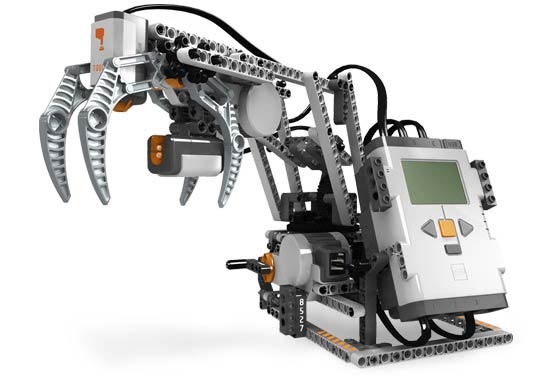
\includegraphics[height=3in]{figure/mindstorm/NXT_machine.png}
    \caption{NXT Machine\label{fig_NXT_machine}}
  \end{center}
\end{figure}
%%%%% END OF FIGURE %%%%%
\noindent
The NXT mindstorm also comes with two other forms, one of these forms is the machine form as shown in Figure
    \ref{fig_NXT_machine}.
In this section, the NXT machine form and the NXT machine demo program will be discussed.
Compared to the NXT vehicle, the NXT machine uses three motors to manipulate its arm and two sensors for detection.
The location and description of the components of the NXT machine is shown in Figure \ref{fig_NXT_machineMOD}.
\newpage
%%%%% START OF FIGURE %%%%%
\begin{figure}[h]
  \begin{center}
    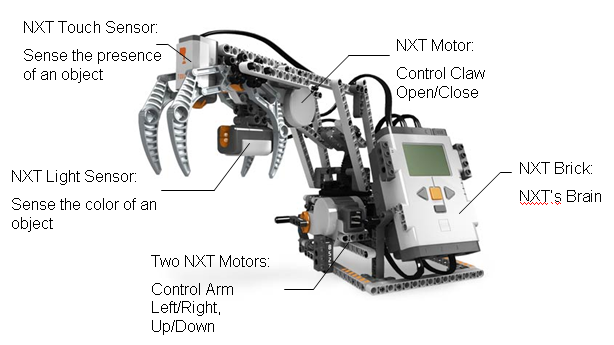
\includegraphics[height=3in]{figure/mindstorm/NXT_machineMOD.png}
    \caption{Components of the NXT Machine\label{fig_NXT_machineMOD}}
  \end{center}
\end{figure}
%%%%% END OF FIGURE %%%%%
\noindent
As shown in Figure \ref{fig_NXT_machineMOD}, one of its motor is responsible for moving its arm left and right.
Another motor is responsible for moving its arm up and down.
The last motor is responsible for controlling its claws open and close.
There are two sensors mounted on the claw, they are the light sensor and the touch sensor.
The NXT machine uses the light sensor to sense the color of the object it is handling.
The NXT uses the touch sensor to sense if it has successfully grabbed an object.
Please use the sensor/motor port configuration shown in Figure \ref{fig_NXT_mach_port} for the
    Ch NXT machine demos programs described in later in this section.
\begin{figure}[h]
  \begin{center}
    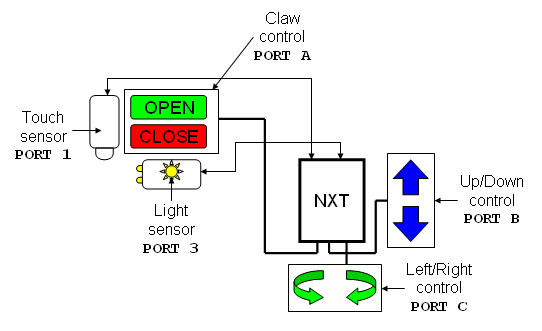
\includegraphics[height=3in]{figure/mindstorm/NXT_mach_port.png}
    \caption{Sensor/Motor configuration of the NXT Machine\label{fig_NXT_mach_port}}
  \end{center}
\end{figure}
\newpage
\subsubsection{Manual Real Time Control Program}
In this section the manual real time control for the NXT machine will be introduced and described.
The manual RTC for the NXT machine allows the user to control the NXT machine manually via the keyboard.
The user interface of the RTC program for the NXT machine is shown in Figure \ref{fig_mach_UI}
\begin{figure}[h]
  \begin{center}
    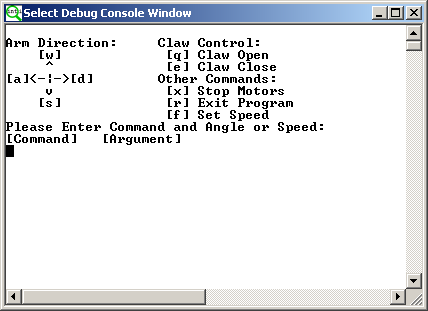
\includegraphics[height=3in]{figure/mindstorm/mach_UI.png}
    \caption{NXT vehicle RTC User Interface \label{fig_mach_UI}}
  \end{center}
\end{figure}
The user interface and the user commands for the NXT machine RTC program is a bit different compared to the
    NXT vehicle RTC program.
Instead of controlling the direction by pressing one key, the user will be required to press a key for
    direction or command, and then enter a number to set the angle or speed.
When a specific key is pressed during the execution of the NXT machine RTC program, the program uses a
    \verb+switch()+ statement to performs a fragment of code that send commands to the NXT to move in 
    a direction or perform a task.
If a directional key or aset speed key has been pressed, program will ask for an user input for a number
    to set the arm to move at an angle or set the speed.
If a discrete task key is pressed, like open or close claw, the program will not ask for an user input for a number.
The list below is the list of commands and a short description of each commands:
\newpage
\begin{itemize}
\item The key \verb+"w"+ is to control the NXT arm to move up.
\item The key \verb+"s"+ is to control the NXT arm to move down.
\item The key \verb+"a"+ is to control the NXT arm to turn left.
\item The key \verb+"d"+ is to control the NXT arm to turn right.
\item The key \verb+"q"+ is to control the NXT claw to open.
\item The key \verb+"e"+ is to control the NXT claw to close.
\item The key \verb+"x"+ is to stop the NXT motors.
\item The key \verb+"r"+ is to exit the manual RTC program.
\item The key \verb+"f"+ is to set the NXT motor speed.
\end{itemize}
The NXT machine RTC program is described in Program 6.
In the rest of this section, we are going to explain important parts of the manual rtc program in detail.
%%%%% Program 6 %%%%%
\verbatiminput{program/mindstorm/machine_rtc.ch}
\begin{center}
Program 6: Manual Real Time Control Program for NXT machine.
\end{center}
%%%%% End of Program 6 %%%%%%
\subsubsection*{How does it work?}
The initialization and the termination of the NXT machine RTC program is very similar to the
   NXT vehicle RTC program.
The biggest difference between the two programs is in the while loop of the program.
In this section, we will focus on how the while() loop of the NXT machine RTC program work internally.

\subsubsection*{While loop}
Similar to the while loop of the NXT vehicle RTC program, the whileloop of the NXT machine RTC program scans for the
    variable quit to see if it is set to 1.
If the 'r' key has been pressed, the variable quit will be set to 1 and the while loop will terminate and the
    machine RTC program will be terminated.
In the while loop, the user will be required to enter different types of command.
Some commands are directional command, where the user needs to enter a number after the command.
Some commands are discrete command, where the user does not need to enter another number.
Instead of simply scanning for a key, the while loop has an additional if statement that scans for which key
    was pressed.
If the key is a directional key or a set speed key, the program ask for the user to input a speed or an angle using
    the \verb+scanf()+ command.
The fragment of the while loop is shown below:
\begin{verbatim}
    while (quit != 1 ) {
        printf("\nEnter command: ");
        dir = _getch();
        if ((dir == 'w') || (dir == 'a') || (dir == 's') 
                || (dir == 'd') || (dir == 'f')){
            printf("  Enter angle or Speed: ");
            scanf("%d", &angle);
        }
        switch (dir){
        
        ...
        
        }
    }
\end{verbatim}
Depending on what key was pressed, the program will run a fragment of code that sends commands to the NXT using the
    \verb+switch()+ command.
\subsubsection*{Directional commands}
The directional movements are controlled using the 'w', 's', 'a', and 'd' keys.
In Figure \ref{fig_mach_UI}, the user interface used arrows to indicate the movement direction and associate
    each direction with a specific key.
\newline
%%% case 'a' %%%
When the key 'a' has been pressed, the \verb+switch()+ function will run the codes for the case 'a'.
The program fragment for case 'a' is shown below:
\begin{verbatim} 
    case 'a': //Arm rotate left. Adjusted angle.
        nxt_motor_rotate(PORT_C, speed, (int)(angle / gearratio));
        break;
\end{verbatim}
In case 'a', the program will run the motor in \verb+PORT_C+ at velocity \verb+speed+, and to an \verb+angle+
    divided by the gear ratio that the user has entered.
Basically, for case 'a' the program will rotate the NXT machine arm left to an adjusted angle that the user
    has entered.
\\
%%% case 'd' %%%
When the key 'd' has been pressed, the \verb+switch()+ function will run the codes for the case 'd'.
The program fragment for case 'd' is shown below:
\begin{verbatim} 
    case 'd': //Arm rotate right. Adjusted angle.
        nxt_motor_rotate(PORT_C, -speed, (int)(angle / gearratio));
        break;
\end{verbatim}
In case 'd', the program will run the motor in \verb+PORT_C+ at velocity \verb+-speed+, and to an \verb+angle+
    divided by the gear ratio that the user has entered.
Basically, for case 'd' the program will rotate the NXT machine arm right to an adjusted angle that the user
    has entered.
\\
%%% case 'w' %%%
When the key 'w' has been pressed, the \verb+switch()+ function will run the codes for the case 'w'.
The program fragment for case 'w' is shown below:
\begin{verbatim} 
    case 'w': //Raise arm up.
        nxt_motor_rotate(PORT_B, speed, angle);
        break;
\end{verbatim}
In case 'w', the program will run the motor in \verb+PORT_B+ at velocity \verb+speed+, and to a prescribed
    \verb+angle+ that the user has entered.
Basically, for case 'w' the program will move the NXT machine arm upward to a prescribed angle that the user
    entered to an angle at a set speed.
\\
%%% case 's' %%%
When the key 's' has been pressed, the \verb+switch()+ function will run the codes for the case 's'.
The program fragment for case 's' is shown below:
\begin{verbatim} 
    case 's': //lower arm down
        nxt_motor_rotate(PORT_B, -speed, angle);
        break;
\end{verbatim}
In case 's', the program will run the motor in \verb+PORT_B+ at velocity \verb+-speed+, and to a prescribed
    \verb+angle+ that the user has entered.
Basically, for case 'w' the program will move the NXT machine arm downward to a prescribed angle that the user
    entered to an angle at set speed.
\\
\subsubsection*{Discrete commands}
The discrete commands are commands that performs a specific task that can either be on or off.
For example, open or close the claw, turn on or off the motors, or quit the program.
For this program, the discrete commands does not require another parameter, so the user does not need to
    input another number for using these commands.
These commands are accessed by entering the 'q', 'e', 'x', 'r' keys.
\newline
%%% case 'q' %%%
When the key 'q' has been pressed, the \verb+switch()+ function will run the codes for the case 'q'.
The program fragment for case 'q' is shown below:
\begin{verbatim} 
    case 'q': //claw open
        nxt_motor(PORT_A, -15, RUN_IDLE);
        sleep(1);
        nxt_motor(PORT_A, 0, RUN_BRAKE);
        break;
\end{verbatim}
In case 'q', the program will run the motor in \verb+PORT_A+ at velocity \verb+-15+, and run idly for 1000
    milliseconds.
Next, the program will hold the position of the motor at that spot, thus keeping the machine claw open.
Basically, for case 'q' the program will open the machine claw.
\\
%%% case 'e' %%%
When the key 'e' has been pressed, the \verb+switch()+ function will run the codes for the case 'e'.
The program fragment for case 'e' is shown below:
\begin{verbatim} 
    case 'e': //claw close
        nxt_motor(PORT_A, 15, RUN_IDLE);
        sleep(1);
        nxt_motor(PORT_A, 0, RUN_BRAKE);	//puts motor in break mode
        break;
\end{verbatim}
In case 'e', the program will run the motor in \verb+PORT_A+ at velocity \verb+15+, and run idly for 1000
    milliseconds.
Next, the program will hold the position of the motor at that spot, thus keeping the machine claw close.
Basically, for case 'e' the program will close the machine claw.
%%% case 'x' %%%
When the key 'x' has been pressed, the \verb+switch()+ function will run the codes for the case 'x'.
The program fragment for case 'x' is shown below:
\begin{verbatim} 
    case 'x': //stop
        nxt_motor_zero();
        nxt_motor(PORT_A, 0, OFF_IDLE);
        nxt_motor(PORT_B, 0, OFF_IDLE);
        nxt_motor(PORT_C, 0, OFF_IDLE);	//puts motor in idle mode
        break;
\end{verbatim}
In case 'x', the program will stop all the motors, and turn the mode to off and idle.
\\
%%% case 'r' %%%
When the key 'r' has been pressed, the \verb+switch()+ function will run the codes for the case 'r'.
The program fragment for case 'r' is shown below:
\begin{verbatim} 
    case 'r': //quit
       printf("\nQuit.");
       quit = 1;
\end{verbatim}
In case 'x', the program will print the string "Quit." and set the variable \verb+quit+ to 1.
By setting the variable \verb+quit+ to 1, the while loop will be terminated, thus quitting the program.
\subsubsection*{Speed setup}
To set the speed of the movement of the arm, the user can enter the key 'f' and enter the speed.
The speed of the motor are in the range of integer of -100 to 100 (negative meaning rotating backward).
The program fragment of case 'f' is shown below:
\begin{verbatim}
    case 'f': //set speed
        speed = angle;
        printf("\nSpeed set to %d.", speed);
\end{verbatim}

\subsubsection*{Using the sensors}
After the switch cases, the while loop will use the sensors to detect if the claw has grabbed an object or not.
If the object has been detected, the program will also try to determine the color of the object using its
    light sensor
In this program, the object that is grabbed is assumed to be a ball, and the color of the ball is assumed to
    be red or blue.
The program fragment for this task is described below:
\begin{verbatim}
    sleep(.200);
    nxt_getsensor(PORT_1);
    if (nxtr.NXT_sensorvalraw[PORT_1] < 500){
        printf("    The Ball was grabbed ");
        nxt_getsensor(PORT_3);
        if (nxtr.NXT_sensorvalraw[PORT_3] < 500){
            printf("and the color is red\n");
        }
        else{
            printf("and the color is blue\n");
        }
    }
\end{verbatim}
In this fragment, the program will sleep for 200 milliseconds and then grab the sensor value stored in
    \verb+PORT_1+ using the \verb+nxt_getsensor()+ command, which is the touch sensor.
Afterward, the if statement checks if the claw has grabbed an object.
If the sensor value for the touch sensor is greater than 500, the touch sensor is not triggered, so there is the NXT
    detected that there is no object in its claw.
If the sensor value for the touch sensor is less than 500, the touch sensor is triggered and the NXT detected that
    the claw has grabbed an object.
\\
When the touch sensor is trigged, the program will continue in the if statement, and the program will 
    prints out that "The Ball was grabbed" in the screen and it get the sensor value stored in
    \verb+PORT_3+, which is the light sensor.
Next, the program will determine the color of the ball using the light sensor value.
If the light sensor value is less than 500, the NXT will detect that the ball that was grabbed is red
    and program will print out "and the color is red".
If the light sensor value is greater than 500, the NXT will detect that the ball that was grabbed is blue
    and program will print out "and the color is blue".
\\
\subsubsection{Autonomous Control Program}
In this section, the autonomous control program for the NXT machine will be introduced.
This autonomous program uses the NXT machine arm to scan it's surrounding.
It performs this task by rotating its arm by an angle step and collect distance data with an
    ultrasonic sensor as it is rotating.
At the end of the program, the collected data will be stored in a data file called 'output.csv', and
    a polar diagram of the data will be display for the user.
The NXT machine automatic control program is described in Program 7.
In the rest of this section, we are going to explain important parts of the automatic control program in detail.
%%%%% Program 7 %%%%%
\verbatiminput{program/mindstorm/machine_auto.ch}
\begin{center}
Program 7: Automatic Control Program for NXT machine.
\end{center}
%%%%% End of Program 7 %%%%%%
Please use the Figure \ref{fig_NXT_machauto_port} to connect your NXT devices for the autonomous
    control program.

\begin{figure}[h]
  \begin{center}
    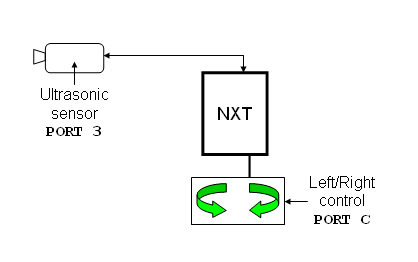
\includegraphics[height=3in]{figure/mindstorm/NXT_machauto_port.png}
    \caption{NXT vehicle RTC User Interface \label{fig_NXT_machauto_port}}
  \end{center}
\end{figure}

\subsubsection*{How does it work?}
In this autonomous program, a for loop is used instead of a while loop.
The for loop will collect data, print out data, and rotate the arm at an angle step for every
    loop.
Some of the parameters are hardcoded in the program, for example, number of loops and angle steps,
    so the user cannot change them as the autonomous program is executed.
These parameters are shown in the program fragment below:
\begin{verbatim}
enum {numpoints=90};    //desired number of data points
const int anglestep=2;	//angle moved between steps
double angle[numpoints];//angle calculated from the tachometer
int distance[numpoints];//data received from the ultrasonic sensor
\end{verbatim}
The variable \verb+numpoints+ determines how many number of times the for loop will run and
    the variable \verb+angles+ determines how much the arm rotates in degrees of angle.
\\
Another feature this program has is the usage information printout described in the program fragment below.
\begin{verbatim}
    printf("\n%d Data points will be collected with a"
        "step size of %d.",numpoints,anglestep);
    printf("\nPlease ensure that the arm can rotate"
        "%d degrees from its current position.",(numpoints*anglestep));
    printf("\nPress any key to continue. Press q at any time to quit.");
    if(getch()=='q'){
        printf("\nQuitting program.");
        sleep(1.500);
        exit(0);
}
\end{verbatim}
In this program fragment, the program will print out how many data point will be collected
    with the angle step size.
Next, it will calculate and print out the full rotation angle of the robot arm and ask the
    user to ensure that the arm can rotate that amount of angle.
Lastly, the program asks the user to continue or quit the program.

\subsubsection*{For loop}
The for loop is the main part of the autonomous program for the NXT machine.
The for loop uses a series of if-else statements to perform data collection and arm movement.
There are three sections for this for loop.
The first section is to collect, store, and print ultrasonic data and angle rotation data.
The second section scans for user input to see if the user has pressed 'q' to quit the program.
The last section is to rotate the arm by an angle step.
The program fragment below is the for loop for the autonomous program for the NXT machine.
\begin{verbatim}
for(i=0;i<numpoints;i++){
    //get sensor data, if success print data, else print error
    if(nxt_getsensor(PORT_3)){
    distance[i]=nxtr.NXT_sensorvalraw[PORT_3];
        if (nxt_gettacho(PORT_C)){
            angle[i]= (nxtr.NXT_motor_pos_cum[PORT_C]*gearratio);
            printf("\nSample: %d,  distance: %d,  Angle: %f",
                i, distance[i],angle[i]);
        }
    }
    else	printf("\nError!");
    //check if q was pressed and if so exit program
    if (!_kbhit){
        if(getch()=='q'){
            printf("\nQuitting program.");
            break;
        }
    }		
    //rotate arm by anglestep (rotate motor anglestep/gear ratio)
    nxt_motor_rotate(PORT_C,100,(anglestep/gearratio));
    sleep(1);
}
\end{verbatim}
The first section of the for loop begins at the line after the first comment and ends at the line
    before the second comment.
The first section begins by getting the ultrasonic sensor data and store it in an array.
If the program is able to retrieve the data, the program will also get the data from the tachometer
    and convert it to angle.
The calculated angle will be stored in another array.
Next, the program will print the sample number, distance detected by ultrasonic sensor, and angle
    rotated by the motor.
If the program is unable to retrieve the data, the program will print error.
\\ \\
The second section of the for loop begins at the line after the second comment and ends at the line
    before the third comment.
In this section, the program checks if a key has been hit by the user, if no key has been hit, this
    section is skipped.
If a key has been hit and it happened to be the 'q' key, the program will print 'Quitting program' and
    the program will be aborted.
\\ \\
The third section of the for loop begins at the line after the third comment and ends at the end of
    the for loop.
In this section, the program controls the motor to rotate at a given angle using the 
    \verb+nxt_motor_rotate()+ command.
Lastly, the program freezes for 1000 milliseconds by using the \verb+Sleep()+ command.
\subsubsection*{Creating and writing data file}
Before the termination of the autonomous control program for the NXT machine, the program creates 
   a data file and stores the collected data in that file.
The program fragment shown below is the program codes for creating and storing a data file for
   the data that was collected:
\begin{verbatim}
stream=fopen("output.csv","w");
for(i=0;i<numpoints;i++){
    fprintf(stream,"%f,%d\n",angle[i],distance[i]);
}
fclose(stream);
\end{verbatim}
In this fragment, the program first creates a file called output.csv and set it to write mode and
    store the file pointer to a variable called stream.
Next, the for loop writes the angle data and the distance data onto the file one set at a time.
At last, the program closes the file by using the function \verb+fclose()+.
\subsubsection*{Plotting data}
In addition to creating and storing a data file, the program also plots a polar diagram for
    the user to visualize the data.
The program fragment below are the commands for plotting the data in a polar diagram.
\begin{verbatim}
//plot data in CH using a polar graph
plot.polarPlot(PLOT_ANGLE_DEG);
plot.data2D(angle,distance);
plot.sizeRatio(1);
plot.grid(PLOT_ON); 
plot.plotting();
\end{verbatim}
In this fragment, the program uses the CPlot class commands to do its plotting.
First, the program use the function \verb+polarPlot()+ to set the plot to polar and degrees in angle.
Next, the program use the function \verb+data2D()+ to insert the collected data onto the polar plot.
Afterward, the program uses the function \verb+sizeRatio()+ function and \verb+grid()+ command to
    correct the size of the plot and to add grid to the plot.
Finally, the program creates the plot by using the function \verb+plotting()+.
%%%%%%%%%%% End of Controlling Your NXT Machine %%%%%%%%%%
\newpage
%%%%%%%%%%% Controlling NXT Humanoid %%%%%%%%%%
\subsection{Controlling NXT Humanoid}
%%%%% START OF FIGURE %%%%%
\begin{figure}[h]
  \begin{center}
    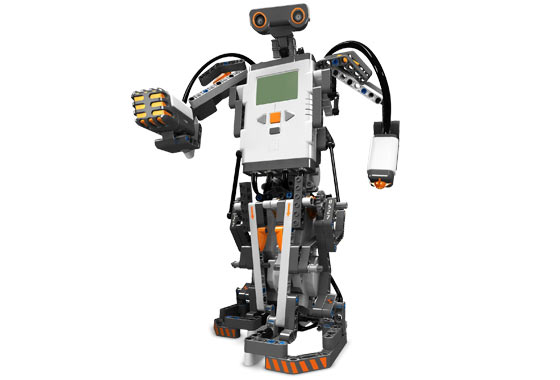
\includegraphics[height=2.5in]{figure/mindstorm/NXT_humanoid.png}
    \caption{NXT Humanoid \label{fig_NXT_humanoid}}
  \end{center}
\end{figure}
\noindent
The third form of the NXT mindstorm is the humanoid form as shown in Figure \ref{fig_NXT_humanoid}
The NXT humanoid uses two of its motors to perform the walking motion.
Also, the NXT humanoid uses its last motor to control the rotation of its head.
The NXT humanoid is equipped with four sensors, a sound sensor on its right hand, a touch sensor on its left hand,
    a light sensor in the back, and an ultrasonic sensor on its head.
In the next section, the real time control program for the NXT humanoid will be discussed.
Please configure your NXT sensors and motors according to Figure \ref{fig_NXT_human_port}
\begin{figure}[h]
  \begin{center}
    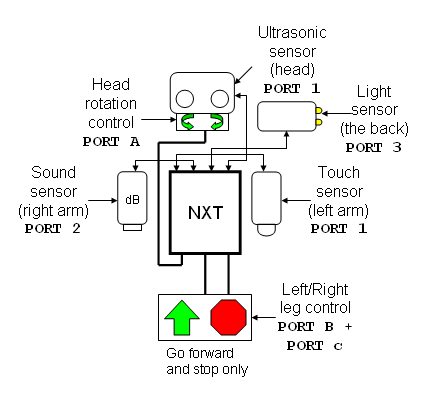
\includegraphics[height=3in]{figure/mindstorm/NXT_human_port.png}
    \caption{Sensor/Motor configuration of the NXT Humanoid\label{fig_NXT_human_port}}
  \end{center}
\end{figure}
\newpage
\subsubsection{Manual Real Time Control Program}
The real time control program of the NXT humanoid is similar to the real time control program of the NXT vehicle.
The RTC program of the NXT humanoid allows the user to control the robot's leg movement and head rotation using the
   keyboard.
In addition, the RTC program allow the user to print out data that has been collected by the NXT sensor.
Figure \ref{fig_human_UI} shows the user interface of the NXT humanoid.
\begin{figure}[h]
  \begin{center}
    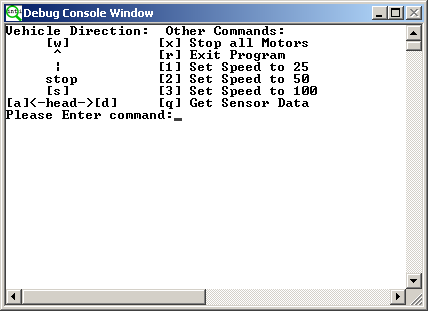
\includegraphics[height=3in]{figure/mindstorm/human_UI.png}
    \caption{NXT Humanoid RTC User Interface \label{fig_human_UI}}
  \end{center}
\end{figure}
The list below is the list of commands:
\begin{itemize}
\item The key \verb+"w"+ is to control the NXT humanoid to walk forward.
\item The key \verb+"s"+ is to control the NXT humanoid to stop.
\item The key \verb+"a"+ is to control the NXT humanoid head to turn left.
\item The key \verb+"d"+ is to control the NXT humanoid head to turn right.
\item The key \verb+"q"+ is to print out sensor data.
\item The key \verb+"x"+ is to stop all of the NXT motors.
\item The key \verb+"r"+ is to exit the RTC program.
\item The number key is to set the NXT motor speed.
\end{itemize}
The NXT humanoid real time control program is described in Program 8.
In the rest of this section, we are going to explain important parts of the manual RTC program in detail.
%%%%% Program 8 %%%%%
\verbatiminput{program/mindstorm/humanoid_rtc.ch}
\begin{center}
Program 8: Manual Real Time Control Program for NXT machine.
\end{center}
%%%%% End of Program 8 %%%%%%
%%%%% END OF FIGURE %%%%%
\subsubsection*{How does it work?}
The the main difference between the RTC program for the NXT humanoid and the NXT vehicle is the content
    in the switch cases.
Other than the switch cases, the while loop of the RTC program is the same as the previous RTC program.
When the key 'r' has been pressed, the \verb+switch()+ function will run the codes for the case 'r'.
In the case 'r', the variable quit will be to 1, which will allow the program to exit the while loop,
    thus quitting the program.
\\
%%% case 'w' %%%
When the key 'w' has been pressed, the \verb+switch()+ function will run the codes for the case 'w'.
The program fragment for case 'w' is shown below:
\begin{verbatim} 
    case 'w': //up
        nxt_motor(PORT_B, speed, RUN_IDLE);
        nxt_motor(PORT_C, speed, RUN_IDLE);
        movemode='w';
        break;
\end{verbatim}
In case 'w', the program will run the motor in \verb+PORT_B+ and \verb+PORT_C+ at velocity \verb+speed+.
Basically, for case 'w' the program will control the NXT humanoid to walk forward at a speed.
\\
%%% case 's' %%%
When the key 's' has been pressed, the \verb+switch()+ function will run the codes for the case 's'.
The program fragment for case 's' is shown below:
\begin{verbatim} 
    case 's': //down
        nxt_motor(PORT_B, 0, OFF_IDLE);
        nxt_motor(PORT_C, 0, OFF_IDLE);
        movemode='s';
        break;
\end{verbatim}
In case 's', the program will stop the motor in \verb+PORT_B+ and \verb+PORT_C+ and turn them to off idle mode.
Basically, for case 's' the program will stop the NXT humanoid from walking forward.
\\
%%% case 'a' %%%
When the key 'a' has been pressed, the \verb+switch()+ function will run the codes for the case 'a'.
The program fragment for case 'a' is shown below:
\begin{verbatim} 
    case 'a': //left
        nxt_motor(PORT_A, -30, RUN_IDLE);
        break;
\end{verbatim}
In case 'a', the program will run the motor in \verb+PORT_A+ at -30 speed.
Basically, for case 'a' the program will rotate the NXT humanoid head left.
\\
%%% case 'd' %%%
When the key 'd' has been pressed, the \verb+switch()+ function will run the codes for the case 'd'.
The program fragment for case 'd' is shown below:
\begin{verbatim} 
    case 'a': //left
        nxt_motor(PORT_A, -30, RUN_IDLE);
        break;
\end{verbatim}
In case 'd', the program will run the motor in \verb+PORT_A+ at 30 speed.
Basically, for case 'd' the program will rotate the NXT humanoid head right.
\\
%%% case 'q' %%%
When the key 'q' has been pressed, the \verb+switch()+ function will run the codes for the case 'q'.
The program fragment for case 'q' is shown below:
\begin{verbatim} 
    case 'q': //print sensor
        printsensor(&nxtr);
        break;
\end{verbatim}
In case 'q', the program will run the function \verb+printsensor()+, which will get sensor data from each data and
    print these data out for the user.
The details of the \verb+printsensor()+ function will be discussed later in this section.
//
%%% case 'x' %%%
When the key 'x' has been pressed, the \verb+switch()+ function will run the codes for the case 'x'.
The program fragment for case 'x' is shown below:
\begin{verbatim} 
    case 'x': //stop
        nxt_motor(PORT_B, 0, OFF_IDLE);
        nxt_motor(PORT_C, 0, OFF_IDLE);
        movemode='x';
        break;
\end{verbatim}
In case 'x', the program will stop all the motors connected to the NXT and set them to off idle mode.
//
\subsubsection*{Printing sensor data}
The function definition for the function \verb+printsensor+ is shown in the program fragment below:
\begin{verbatim}
int printsensor(struct nxt_remote *nxtr){
    int touch=0;
    int ultra=0;
    int sound=0;
    int light=0;

    nxt_getsensor(PORT_1);
    nxt_getsensor(PORT_2);
    nxt_getsensor(PORT_3);
    nxt_getsensor(PORT_4);
    touch=nxtr->NXT_sensorvalraw[PORT_1];
    sound=nxtr->NXT_sensorvalraw[PORT_2];
    light=nxtr->NXT_sensorvalraw[PORT_3];
    ultra=nxtr->NXT_sensorvalraw[PORT_4];

    if (touch<500)
        printf("\n\n\nThe touch sensor has been activated.\n",touch);
    else
        printf("\nThe touch sensor has not been activated.\n");
    
    printf("The distance reported by the ultrasonic sensor is %d.\n",ultra);
    /*
    if (light<500)  printf("\nThe touch sensor has been activated\n");
    else    printf("\nThe touch sensor has been activated\n");
    */
    printf("The light level is %d.\n",light);
    printf("The Sound level is %dDb\n\n\n",sound);
    
    //GUI display
    printf("Vehicle Direction:  Other Commands:");
    printf("\n     [w]           [x] Stop all Motors");
    printf("\n      ^            [r] Exit Program");
    printf("\n      |            [1] Set Speed to 25");
    printf("\n     stop          [2] Set Speed to 50");
    printf("\n     [s]           [3] Set Speed to 75");
    printf("\n[a]<-head->[d]     [q] Get Sensor Data\n");
    printf("Please Enter command:");
    return(1);
}
\end{verbatim}
In the beginning of this function, the program get sensor data from each sensor and store them in its corresponding
    variable.
Next, if else statements are used to print the correct statement if the sensor is triggered or not.
For example, if the touch sensor is triggered, the sensor data retrieved is below 500, then the program will
    print 'The touch sensor has been activated'.
Next, the program will print out the distance collected by the ultrasonic sensor, then the light sensor and lastly
    the sound sensor.
Finally, the function prints the user interface again for the user to read.

%%%%%%%%%%% End of Controlling Your NXT Humanoid %%%%%%%%%%
\newpage
%%%%%%%%%% APPENDIX %%%%%%%%%%
\section{Appendix}

%%%%%%%%%% User Functions %%%%%%%%%%
\subsection{User Functions}
\begin{tabular}{ | l | p{11cm} |}\hline
Functions & Description\\
\hline
\verb+nxt_connect()+ 		& Connects to the Mindstorms NXT using blue tooth.\\
\verb+nxt_forward()+		& Moves the NXT vehicle forward.\\
\verb+nxt_backward()+		& Moves the NXT vehicle backward.\\
\verb+nxt_turnleft()+		& Turns the NXT vehicle left.\\
\verb+nxt_turnright()+		& Turns the NXT vehicle right.\\
\verb+nxt_rotateleft()+		& Rotates the NXT vehicle to the left in place.\\
\verb+nxt_rotateright()+	& Rotates the NXT vehicle to the right in place.\\
\verb+nxt_stop()+	        & Stops all motors on the NXT.\\
\verb+nxt_motor()+			& Sets the motor output for NXT.\\
\verb+nxt_motor_rotate()+ 	& Rotate the motor for NXT for given degree.\\
\verb+nxt_setsensor()+		& Set up the sensors to collect data for the NXT.\\
\verb+nxt_getsensor()+		& Get sensor data from NXT.\\
\verb+nxt_printmess()+ 		& Prints the last message send to or receive from NXT.\\
\verb+nxt_disconnect()+ 	& Disconnect the NXT.\\
\verb+nxt_gettacho()+		& Get tachometer counts from NXT.\\
\verb+nxt_motor_zero()+		& Reset tachometer count to zero for all motors.\\
\hline
\end{tabular}
%%%%%%%%%% End of Functions %%%%%%%%%%

%%%%%%%%%% Macros %%%%%%%%%%
\subsection{Functions}
\begin{tabular}{ | l | l | p{10cm} |}\hline
Name 			&	Value	&	Description\\
\hline
				&			&	Motor Macros\\
\hline
Motor Ports:	&			&	\\
\hline
\verb+PORT_A+	&	0		&	Select output PORT A.\\
\verb+PORT_B+	&	1		&	Select output PORT B.\\
\verb+PORT_C+	&	2		&	Select output PORT C.\\
\hline
Motor Mode:		&			&	\\
\hline
\verb+RUN_IDLE+	&	0		&	Sets motor to run, idle.\\
\verb+RUN_BRAKE+&	1		&	Sets motor to run, brake.\\
\verb+OFF_IDLE+	&	3		&	Sets motor to off, idle.\\
\hline
				&			&	Sensor Macros\\
\hline
Sensor Ports:	&			&	\\
\hline
\verb+PORT_1+	&	0		&	Select sensor input PORT 1.\\
\verb+PORT_2+	&	1		&	Select sensor input PORT 2.\\
\verb+PORT_3+	&	2		&	Select sensor input PORT 3.\\
\verb+PORT_4+	&	3		&	Select sensor input PORT 4.\\
\hline
Sensor Type:	&			&	\\
\hline
\verb+TOUCH+		&	1	&	Sets to Touch sensor.\\
\verb+TEMPERATURE+	&	2	&	Sets to Temperature Sensor.\\
\verb+LIGHT_ACTIVE+	&	5	&	Sets to Light Sensor in active mode(LED on).\\
\verb+LIGHT_INACTIVE+ &	6	&	Sets to Light Sensor in inactive mode(LED off).\\
\verb+SOUND_DB+		&	7	&	Sets to Sound Sensor in dB.\\
\verb+SOUND_DBA+	&	8	&	Sets to Sound Sensor in dBa.\\
\verb+ULTRASONIC+	&	11	&	Sets to Ultrasonic Sensor.\\
\hline
Sensor Mode:	&			&	\\
\hline
RAWMODE			&	0		&	\\	 
BOOLEANMODE		&	50	 	&	\\
\hline
\end{tabular}
%%%%%%%%%% End of Macros %%%%%%%%%%
\hrule
\newpage

%%%%% nxt_connect %%%%%
\section*{nxt\_connect}

\subsubsection*{Synopsis}
\begin{verbatim}
#include <ch_nxt.h>
int nxt_connect(struct nxt_remote *nxt_user);
\end{verbatim}

\subsubsection*{Purpose}
Connects to the Mindstorms NXT using bluetooth.

\subsubsection*{Return Value}
Returns 1 if successful, returns 0 if failed.

\subsubsection*{Parameters}
\begin{tabular}{ l | p{12cm} }
Parameter			& Description\\ \hline
\verb+*nxt_user+	& The address of the structure \verb+nxt_remote+
					  that the user created in the main function.
\end{tabular}

\subsubsection*{Description}
This function connects to the Mindstorms NXT using blue tooth. The parameter \verb+ *nxt_user+ is the address of the structure \verb+nxt_remote+ that stores the input/output data and port addresses. The function will return 1 if successful and return 0 if failed.

\subsubsection*{Example}
\begin{verbatim}
#include <ch_nxt.h> 
#include <stdio.h>

struct nxt_remote nxtr;
if (!nxt_connect(&nxtr)){
    printf("Connection to NXT has failed.");
    exit(0);
}
    
nxt_disconnect();
\end{verbatim}

\subsubsection*{Output}
None 
\\
%%%%% END OF nxt_connect %%%%%

\hrule
\newpage

%%%%% nxt_forward %%%%%
\section*{nxt\_forward}

\subsubsection*{Synopsis}
\begin{verbatim}
#include <ch_nxt.h>
int nxt_forward(int speed);
\end{verbatim}

\subsubsection*{Purpose}
Move the NXT vehicle forward at the specified speed.

\subsubsection*{Return Value}
Returns 1 if successful, returns 0 if failed.

\subsubsection*{Parameters}
\begin{tabular}{ l | p{12cm} }
Parameter			& Description\\ \hline
\verb+speed+	    & Speed of the motors, (range is from 1 to 100).
\end{tabular}

\subsubsection*{Description}
The function is meant for use only with the NXT vehicle designed robot, 
and may not function correctly with other designs. The function sets the 
output of the motors based on the parameter \verb+speed+. The values are 
based off of the speed that the individual motors of the NXT can be set to. 
The NXT will continue to move forward at the set speed until the motors are 
stopped.

\subsubsection*{Example}
\begin{verbatim}
#include <ch_nxt.h> 
#include <stdio.h>
#include <unistd.h>

int speed;
struct nxt_remote nxtr;
if (!nxt_connect(&nxtr)){
    printf("Connection to NXT has failed.");
    exit(0);
}
    
nxt_forward(speed);
sleep(5);
nxt_stop();

nxt_disconnect();
\end{verbatim}

\subsubsection*{Output}
None 
\\
%%%%% END OF nxt_forward %%%%%

\hrule
\newpage

%%%%% nxt_backward %%%%%
\section*{nxt\_backward}

\subsubsection*{Synopsis}
\begin{verbatim}
#include <ch_nxt.h>
int nxt_backward(int speed);
\end{verbatim}

\subsubsection*{Purpose}
Move the NXT vehicle backward at the specified speed.

\subsubsection*{Return Value}
Returns 1 if successful, returns 0 if failed.

\subsubsection*{Parameters}
\begin{tabular}{ l | p{12cm} }
Parameter			& Description\\ \hline
\verb+speed+	    & Speed of the motors, (range is from 1 to 100).
\end{tabular}

\subsubsection*{Description}
The function is meant for use only with the NXT vehicle designed robot, 
and may not function correctly with other designs. The function sets the 
output of the motors based on the parameter \verb+speed+. The values are 
based off of the speed that the individual motors of the NXT can be set to. 
The NXT will continue to move backward at the set speed until the motors 
are stopped.

\subsubsection*{Example}
\begin{verbatim}
#include <ch_nxt.h> 
#include <stdio.h>
#include <unistd.h>

int speed;
struct nxt_remote nxtr;
if (!nxt_connect(&nxtr)){
    printf("Connection to NXT has failed.");
    exit(0);
}

nxt_backward(speed);
sleep(5);
nxt_stop();
    
nxt_disconnect();
\end{verbatim}

\subsubsection*{Output}
None 
\\
%%%%% END OF nxt_backward %%%%%

\hrule
\newpage

%%%%% nxt_turnleft %%%%%
\section*{nxt\_turnleft}

\subsubsection*{Synopsis}
\begin{verbatim}
#include <ch_nxt.h>
int nxt_turnleft(int speed);
\end{verbatim}

\subsubsection*{Purpose}
Move the NXT vehicle forward and turn left at the specified speed.

\subsubsection*{Return Value}
Returns 1 if successful, returns 0 if failed.

\subsubsection*{Parameters}
\begin{tabular}{ l | p{12cm} }
Parameter			& Description\\ \hline
\verb+speed+	    & Speed of the motors, (range is from 1 to 100).
\end{tabular}

\subsubsection*{Description}
The function is meant for use only with the NXT vehicle designed robot, 
and may not function correctly with other designs. The function sets the 
right wheel to the \verb+speed+ value and the left wheel to 0.7 * 
\verb+speed+ value. The motors will continue to rotate until a motor speed 
is changed or the motors are stopped.

\subsubsection*{Example}
\begin{verbatim}
#include <ch_nxt.h> 
#include <stdio.h>
#include <unistd.h>

int speed;
struct nxt_remote nxtr;
if (!nxt_connect(&nxtr)){
    printf("Connection to NXT has failed.");
    exit(0);
}
    
nxt_turnleft(speed);
sleep(3);
nxt_stop();

nxt_disconnect();
\end{verbatim}

\subsubsection*{Output}
None 
\\
%%%%% END OF nxt_turnleft %%%%%

\hrule
\newpage

%%%%% nxt_turnright %%%%%
\section*{nxt\_turnright}

\subsubsection*{Synopsis}
\begin{verbatim}
#include <ch_nxt.h>
int nxt_turnright(int speed);
\end{verbatim}

\subsubsection*{Purpose}
Move the NXT vehicle forward and turn right at the specified speed.

\subsubsection*{Return Value}
Returns 1 if successful, returns 0 if failed.

\subsubsection*{Parameters}
\begin{tabular}{ l | p{12cm} }
Parameter			& Description\\ \hline
\verb+speed+	    & Speed of the motors, (range is from 1 to 100).
\end{tabular}

\subsubsection*{Description}
The function is meant for use only with the NXT vehicle designed robot, 
and may not function correctly with other designs. The function sets the 
left wheel to the \verb+speed+ value and the right wheel to 0.7 * 
\verb+speed+ value. The motors will continue to rotate until a motor speed 
is changed or the motors are stopped.


\subsubsection*{Example}
\begin{verbatim}
#include <ch_nxt.h> 
#include <stdio.h>
#include <unistd.h>

int speed;
struct nxt_remote nxtr;
if (!nxt_connect(&nxtr)){
    printf("Connection to NXT has failed.");
    exit(0);
}
    
nxt_turnright(speed);
sleep(3);
nxt_stop();

nxt_disconnect();
\end{verbatim}

\subsubsection*{Output}
None 
\\
%%%%% END OF nxt_turnright %%%%%

\hrule
\newpage

%%%%% nxt_rotateleft %%%%%
\section*{nxt\_rotateleft}

\subsubsection*{Synopsis}
\begin{verbatim}
#include <ch_nxt.h>
int nxt_rotateleft(int speed);
\end{verbatim}

\subsubsection*{Purpose}
Rotate the NXT vehicle to the left in place at the specified speed.

\subsubsection*{Return Value}
Returns 1 if successful, returns 0 if failed.

\subsubsection*{Parameters}
\begin{tabular}{ l | p{12cm} }
Parameter			& Description\\ \hline
\verb+speed+	    & Speed of the motors, (range is from 1 to 100).
\end{tabular}

\subsubsection*{Description}
The function is meant for use only with the NXT vehicle designed robot, 
and may not function correctly with other designs. The right wheel is 
set to the value of \verb+speed+ and the left wheel is set to 
negative \verb+speed+.  The NXT vehicle will continue to rotate in 
place until until a motor speed is changed or the motors are stopped.

\subsubsection*{Example}
\begin{verbatim}
#include <ch_nxt.h> 
#include <stdio.h>
#include <unistd.h>

int speed;
struct nxt_remote nxtr;
if (!nxt_connect(&nxtr)){
    printf("Connection to NXT has failed.");
    exit(0);
}
    
nxt_rotateleft(speed);
sleep(3);
nxt_stop();

nxt_disconnect();
\end{verbatim}

\subsubsection*{Output}
None 
\\
%%%%% END OF nxt_rotateleft %%%%%

\hrule
\newpage

%%%%% nxt_rotateright %%%%%
\section*{nxt\_rotateright}

\subsubsection*{Synopsis}
\begin{verbatim}
#include <ch_nxt.h>
int nxt_rotateright(int speed);
\end{verbatim}

\subsubsection*{Purpose}
Rotate the NXT vehicle to the right in place at the specified speed.

\subsubsection*{Return Value}
Returns 1 if successful, returns 0 if failed.

\subsubsection*{Parameters}
\begin{tabular}{ l | p{12cm} }
Parameter			& Description\\ \hline
\verb+speed+	    & Speed of the motors, (range is from 1 to 100).
\end{tabular}

\subsubsection*{Description}
The function is meant for use only with the NXT vehicle designed robot, 
and may not function correctly with other designs. The left wheel is 
set to the value of \verb+speed+ and the right wheel is set to 
negative \verb+speed+.  The NXT vehicle will continue to rotate in 
place until until a motor speed is changed or the motors are stopped.

\subsubsection*{Example}
\begin{verbatim}
#include <ch_nxt.h> 
#include <stdio.h>
#include <unistd.h>

int speed;
struct nxt_remote nxtr;
if (!nxt_connect(&nxtr)){
    printf("Connection to NXT has failed.");
    exit(0);
}
    
nxt_rotateright(speed);
sleep(3);
nxt_stop();

nxt_disconnect();
\end{verbatim}

\subsubsection*{Output}
None 
\\
%%%%% END OF nxt_rotateright %%%%%

\hrule
\newpage

%%%%% nxt_stop %%%%%
\section*{nxt\_stop}

\subsubsection*{Synopsis}
\begin{verbatim}
#include <ch_nxt.h>
int nxt_stop();
\end{verbatim}

\subsubsection*{Purpose}
Stops all motors on the Mindstorm NXT.

\subsubsection*{Return Value}
Returns 1 if successful, returns 0 if failed.

\subsubsection*{Parameters}
None

\subsubsection*{Description}
The function stops all the motors on the Mindstorm NXT. This 
function should not be used if you only want to stop one motor in 
your program.

\subsubsection*{Example}
\begin{verbatim}
#include <ch_nxt.h> 
#include <stdio.h>
#include <unistd.h>

int speed;
struct nxt_remote nxtr;
if (!nxt_connect(&nxtr)){
    printf("Connection to NXT has failed.");
    exit(0);
}
    
nxt_forward(speed);
sleep(3);
nxt_stop();

nxt_rotateright(speed);
sleep(3);
nxt_stop();

nxt_disconnect();
\end{verbatim}

\subsubsection*{Output}
None 
\\
%%%%% END OF nxt_stop %%%%%

\hrule
\newpage

%%%%% nxt_motor %%%%%
\section*{nxt\_motor}

\subsubsection*{Synopsis}
\begin{verbatim}
#include <ch_nxt.h>
int nxt_motor(int port, int speed, int brake);
\end{verbatim}

\subsubsection*{Purpose}
Sets the motor output for NXT.

\subsubsection*{Return Value}
Returns 1 if successful, returns 0 if failed.

\subsubsection*{Parameters}
\begin{tabular}{ l | p{12cm} }
Parameter		& Description\\ \hline
\verb+port+		& motor port connection to NXT.\\
\verb+speed+	& Speed of the motor, (range is from -100 to 100).\\
\verb+brake+	& The mode of the motor.
\end{tabular}

\subsubsection*{Description}
This function sets the motor output for NXT. The parameter \verb+port+ indicate which motor port you would like to control. The \verb+MACRO+s available for the parameter \verb+port+ are \verb+PORT_A+, 	\verb+PORT_B+, and \verb+PORT_C+, which refers to Port A, Port B, and Port C of the NXT brick. The speed of the motor is set by the parameter \verb+speed+. The minimum value for \verb+speed+ is -100, which refer to run motor at full speed in reverse. The maximum value for \verb+speed+ is 100, which refer to run motor at full speed forward. If the \verb+speed+ is set to zero, then the motor will not run. The mode of the motor is set by parameter \verb+brake+. The \verb+MACRO+s available for parameter are \verb+RUN_IDLE+, \verb+RUN_BRAKE+, \verb+OFF_IDLE+. The function will return 1 if successful and return 0 if failed.

\subsubsection*{Example}
\begin{verbatim}
#include <ch_nxt.h> 
#include <stdio.h>

struct nxt_remote nxtr;
if (!nxt_connect(&nxtr)){
    printf("Connection to NXT has failed.");
    exit(0);
}
int speed = 25;
nxt_motor(PORT_B, speed, RUN_IDLE);
nxt_motor(PORT_C, speed, RUN_IDLE);
//Allow the NXT to run for the next 5 seconds
Sleep(5000);
nxt_disconnect();    
\end{verbatim}

\subsubsection*{Output}
None 
\\
%%%%% END OF nxt_motor %%%%%

\hrule
\newpage

%%%%% nxt_motor_rotate %%%%%
\section*{nxt\_motor\_rotate}

\subsubsection*{Synopsis}
\begin{verbatim}
#include <ch_nxt.h>
int nxt_motor_rotate(int port, int speed, int degrees);
\end{verbatim}

\subsubsection*{Purpose}
Rotate the motor for NXT for given degree.

\subsubsection*{Return Value}
Returns 1 if successful, returns 0 if failed.

\subsubsection*{Parameters}
\begin{tabular}{ l | p{12cm} }
Parameter		& Description\\ \hline
\verb+port+		& motor port connection to NXT.\\
\verb+speed+	& Speed of the motor, (range is from -100 to 100).\\
\verb+degrees+	& The degree which the motor will rotate.
\end{tabular}

\subsubsection*{Description}
This function will rotate a motor at a given speed at a given degree. 
The parameter \verb+port+ indicate which motor should the NXT set output to. 
The \verb+MACRO+s available for the parameter \verb+port+ are \verb+PORT_A+, 
\verb+PORT_B+, and \verb+PORT_C+, which refers to Port A, Port B, and Port C of the NXT brick. 
The speed of the motor is set by the parameter \verb+speed+. 
The minimum value for \verb+speed+ is -100, which refer to run motor at full speed in reverse. 
The maximum value for \verb+speed+ is 100, which refer to run motor at full speed forward. 
The degree which the motor will rotate is set by the parameter \verb+degree+. 
The function will return 1 if successful and return 0 if failed.

\subsubsection*{Example}
\begin{verbatim}
#include <ch_nxt.h> 
#include <stdio.h>

struct nxt_remote nxtr;
if (!nxt_connect(&nxtr)){
    printf("Connection to NXT has failed.");
    exit(0);
}
int speed = 25;
int degree = 360;
nxt_motor_rotate(PORT_B, speed, degree);
nxt_motor_rotate(PORT_C, speed, degree);
//Allow the NXT to run for the next 5 seconds
Sleep(5000);    
nxt_disconnect();  
\end{verbatim}

\subsubsection*{Output}
None 
\\
%%%%% END OF nxt_motor_rotate %%%%%

\hrule
\newpage

%%%%% nxt_setsensor %%%%%
\section*{nxt\_setsensor}

\subsubsection*{Synopsis}
\begin{verbatim}
#include <ch_nxt.h>
int nxt_setsensor(int port, int sensortype, int sensormode)
\end{verbatim}

\subsubsection*{Purpose}
Set up the sensors to collect data for the NXT.

\subsubsection*{Return Value}
Returns 1 if successful, returns 0 if failed.

\subsubsection*{Parameters}
\begin{tabular}{ l | p{12cm} }
Parameter			& Description\\ \hline
\verb+port+			& sensor input port connection to NXT.\\
\verb+sensortype+	& Type of sensor that is connected.\\
\verb+sensormode+	& Sensor mode.
\end{tabular}

\subsubsection*{Description}
This function set up the sensors to collect data for the NXT. 
The parameter \verb+port+ select which port is configured within the function. 
The \verb+MACRO+s available for the parameter \verb+port+ are \verb+PORT_1+, 	\verb+PORT_2+, \verb+PORT_3+, and \verb+PORT_4+, 	which refers to Port 1, Port 2, Port 3, and Port 4 of the NXT brick. The type of sensor can be configured using the parameter \verb+sensortype+. The \verb+MACRO+s available for parameter \verb+sensortype+ are \verb+TOUCH+, \verb+TEMPERATURE+, 	\verb+LIGHT_ACTIVE+, \verb+LIGHT_INACTIVE+, \verb+SOUND_DB+, \verb+SOUND_DBA+, and \verb+UNLTRASONIC+. The mode for the sensor can be selected with the parameter \verb+sensormode+. The \verb+MACRO+s available for \verb+sensormode+ are \verb+RAWMODE+ and \verb+BOOLEANMODE+. The function will return 1 if successful and return 0 if failed.
\subsubsection*{Example}
\begin{verbatim}
#include <ch_nxt.h> 
#include <stdio.h>

struct nxt_remote nxtr;
if (!nxt_connect(&nxtr)){
    printf("Connection to NXT has failed.");
    exit(0);
}
int status_1=2;
int status_2=2;
    
status_1=nxt_setsensor(PORT_1,TOUCH,BOOLEANMODE);
status_2=nxt_setsensor(PORT_4,ULTRASONIC,RAWMODE);
if(status_1==0){
    printf("Connection to touch sensor has failed");
}
if(status_2==0){
    printf("Connection to ultrasonic sensor has failed");
}
    
nxt_disconnect();
\end{verbatim}

\subsubsection*{Output}
None 
\\
%%%%% END OF nxt_setsensor %%%%%

\hrule
\newpage

%%%%% nxt_getsensor %%%%%
\section*{nxt\_getsensor}

\subsubsection*{Synopsis}
\begin{verbatim}
#include <ch_nxt.h>
nxt_getsensor(int port);
\end{verbatim}

\subsubsection*{Purpose}
Retrieve sensor data from NXT.

\subsubsection*{Return Value}
Returns 1 if successful, returns 0 if failed.

\subsubsection*{Parameters}
\begin{tabular}{ l | p{12cm} }
Parameter			& Description\\ \hline
\verb+port+			& The sensor port that you want to gather data from. 
\end{tabular}

\subsubsection*{Description}
This function allow the user to retrieve sensor data from a selected port. The parameter \verb+port+ allow the user to select which sensor to gather data from. The \verb+MACRO+s available for the parameter \verb+port+ are \verb+PORT_1+, \verb+PORT_2+, \verb+PORT_3+, and \verb+PORT_4+, which refers to Port 1, Port 2, Port 3, and Port 4 of the NXT brick. The result is stored in \verb+NXT_sensorvalraw[port]+.
The function will return 1 if successful and return 0 if failed.

\subsubsection*{Example}
\begin{verbatim}
#include <ch_nxt.h> 
#include <stdio.h>

struct nxt_remote nxtr;
if (!nxt_connect(&nxtr)){
    printf("Connection to NXT has failed.");
    exit(0);
}
int status_1=2;
int status_2=2;
    
status_1=nxt_setsensor(PORT_1,TOUCH,BOOLEANMODE);
status_2=nxt_setsensor(PORT_4,ULTRASONIC,RAWMODE);
if(status_1==0){
    printf("Connection to touch sensor has failed");
}
if(status_2==0){
    printf("Connection to ultrasonic sensor has failed");
}
//get sensor data
nxt_getsensor(PORT_1);
nxt_getsensor(PORT_4);
    
//store sensor data in variables
int port_1_data;
int port_4_data;
port_1_data = nxtr.NXT_sensorvalraw[PORT_1];
port_4_data = nxtr.NXT_sensorvalraw[PORT_4];
    
nxt_disconnect();
\end{verbatim}

\subsubsection*{Output}
None 
\\
%%%%% END OF nxt_getsensor %%%%%

\hrule
\newpage
%%%%% nxt_printmess() %%%%%
\section*{nxt\_printmess}

\subsubsection*{Synopsis}
\begin{verbatim}
#include <ch_nxt.h>
int nxt_printmess();
\end{verbatim}

\subsubsection*{Purpose}
Print the last message sent to or receive from the NXT.

\subsubsection*{Return Value}
Returns 1 if successful, returns 0 if failed.

\subsubsection*{Parameters}
None

\subsubsection*{Description}
Allow the user to print the last message sent to or receive from the NXT.
The function will return 1 if successful and return 0 if failed.

\subsubsection*{Example}
\begin{verbatim}
#include <ch_nxt.h> 
#include <stdio.h>

struct nxt_remote nxtr;
if (!nxt_connect(&nxtr)){
    printf("Connection to NXT has failed.");
    exit(0);
}
nxt_printmess();    
\end{verbatim}

\subsubsection*{Output}
None 
\\
%%%%% END OF nxt_printmess %%%%%

\hrule
\newpage
%%%%% nxt_disconnect %%%%%
\section*{nxt\_disconnect}

\subsubsection*{Synopsis}
\begin{verbatim}
#include <ch_nxt.h>
int nxt_disconnect();
\end{verbatim}

\subsubsection*{Purpose}
Disconnect the NXT from your computer.

\subsubsection*{Return Value}
Returns 1 if successful, returns 0 if failed.

\subsubsection*{Parameters}
None

\subsubsection*{Description}
This function allow the user to disconnect the NXT from your computer. This function also turns all motors to off/idle, and turns all sensors to none. The function will return 1 if successful and return 0 if failed.

\subsubsection*{Example}
\begin{verbatim}
#include <ch_nxt.h> 
#include <stdio.h>

struct nxt_remote nxtr;
if (!nxt_connect(&nxtr)){
    printf("Connection to NXT has failed.");
    exit(0);
}
//Disconnect NXT
nxt_disconnect();    
\end{verbatim}

\subsubsection*{Output}
None 
\\
%%%%% END OF nxt_disconnect %%%%%

\hrule
\newpage
%%%%% nxt_gettacho() %%%%%
\section*{nxt\_gettacho}

\subsubsection*{Synopsis}
\begin{verbatim}
#include <ch_nxt.h>
int nxt_gettacho(int port);
\end{verbatim}

\subsubsection*{Purpose}
Retrieve the tachometer count for the motor.

\subsubsection*{Return Value}
Returns 1 if successful, returns 0 if failed.

\subsubsection*{Parameters}
\begin{tabular}{ l | p{12cm} }
Parameter			& Description\\ \hline
\verb+port+			& The motor port that you want to gather tachometer count from. 
\end{tabular}

\subsubsection*{Description}
This function allow the user to retrieve the tachometer count for the motor. The parameter \verb+port+ indicate which motor should the system gather tachometer count from. The \verb+MACRO+s available for the parameter \verb+port+ are \verb+PORT_A+, \verb+PORT_B+, and \verb+PORT_C+, which refers to Port A, Port B, and Port C of the NXT brick. The result is stored in \verb+nxt_motor_pos_raw[port]+ and \verb+nxt_motor_pos_cum[port]+. The function will return 1 if successful and return 0 if failed.

\subsubsection*{Example}
\begin{verbatim}
#include <ch_nxt.h> 
#include <stdio.h>

struct nxt_remote nxtr;
if (!nxt_connect(&nxtr)){
    printf("Connection to NXT has failed.");
    exit(0);
}
int speed = 25;
int degree = 360;
int count;
    
//Rotate motor
nxt_motor_rotate(PORT_B, speed, degree);
//Allow the NXT to run for the next 5 seconds
Sleep(5000);    
//Get tachometer count
nxt_gettacho(PORT_B);
    
//Store tachometer count in variable
count = nxtr.NXT_motor_pos_cum[PORT_B];
    
nxt_disconnect();
\end{verbatim}

\subsubsection*{Output}
None 
\\
%%%%% END OF nxt_gettacho %%%%%

\hrule
\newpage
%%%%% nxt_motor_zero() %%%%%
\section*{nxt\_motor\_zero}

\subsubsection*{Synopsis}
\begin{verbatim}
#include <ch_nxt.h>
int nxt_motor_zero();
\end{verbatim}

\subsubsection*{Purpose}
Reset the tachometer count for all motors.

\subsubsection*{Return Value}
Returns 1 if successful, returns 0 if failed.

\subsubsection*{Parameters}
None

\subsubsection*{Description}
This function allow the user to reset the tachometer count for all of the motor. The function will return 1 if successful and return 0 if failed.

\subsubsection*{Example}
\begin{verbatim}
#include <ch_nxt.h> 
#include <stdio.h>

struct nxt_remote nxtr;
if (!nxt_connect(&nxtr)){
    printf("Connection to NXT has failed.");
    exit(0);
}
int speed = 25;
int degree = 360;
int count;

//Rotate motor
nxt_motor_rotate(PORT_B, speed, degree);
//Allow the NXT to run for the next 5 seconds
Sleep(5000);    
//Get tachometer count
nxt_gettacho(PORT_B);
    
//Store tachometer count in variable
count = nxtr.NXT_motor_pos_cum[PORT_B];
    
//Reset the tachometer count
nxt_motor_zero();
nxt_disconnect();
\end{verbatim}

\subsubsection*{Output}
None 
\\
%%%%% END OF nxt_motor_zero %%%%%
%%%%%%%%%% End of APPENDIX %%%%%%%%%%

\end{document}
